% !TEX TS-program = lualatex
% Copyright (C)  2026 Alain Matthes
% This work may be distributed and/or modified under the
% conditions of the LaTeX Project Public License, either version 1.3
% of this license or (at your option) any later version.
% The latest version of this license is in
%   http://www.latex-project.org/lppl.txt
% and version 1.3 or later is part of all distributions of LaTeX
% version 2005/12/01 or later.
% This work has the LPPL maintenance status `maintained'.
% The Current Maintainer of this work is Alain Matthes

% TKZdoc-fn-main : 中文文档 tkz-fn.

\documentclass[DIV         = 14,
               fontsize    = 10,
               index       = totoc,
               twoside,
               headings    = small
               ]{tkz-doc}
\usepackage{etoc}
\gdef\tkznameofpack{tkz-fn}
\gdef\tkzversionofpack{1.00c}
\gdef\tkzdateofpack{2026/10/19}
\gdef\tkznameofdoc{doc-tkz-fn}
\gdef\tkzdateofdoc{2026/10/19}
\gdef\tkzversionofdoc{1.00c}
\gdef\tkzauthorofpack{Alain Matthes}
\gdef\tkzadressofauthor{}
\gdef\tkznamecollection{AlterMundus}
\gdef\tkzurlauthor{http://altermundus.fr}
\gdef\tkzurlauthorcom{http://altermundus.fr}
\gdef\tkzengine{lualatex}
\usepackage{tkz-tab}
\usepackage[english]{alterqcm}
\usepackage{tkz-fn}
\usetikzlibrary{arrows,patterns,shapes.geometric}
\usepackage[colorlinks]{hyperref}
\hypersetup{
      linkcolor=Gray,
      citecolor=Green,
      filecolor=Mulberry,
      urlcolor=NavyBlue,
      menucolor=Gray,
      runcolor=Mulberry,
      linkbordercolor=Gray,
      citebordercolor=Green,
      filebordercolor=Mulberry,
      urlbordercolor=NavyBlue,
      menubordercolor=Gray,
      runbordercolor=Mulberry,
      pdfsubject={用 Lua 绘制函数图像},
      pdfauthor={\tkzauthorofpack},
      pdftitle={\tkznameofpack},
      pdfkeywords={tikz, pgf, lua, lualatex, graphic, maths, graph,
      function, tangent, area},
      pdfcreator={\tkzengine}
}
\usepackage{url}
\def\UrlFont{\small\ttfamily}

\usepackage{fontspec}
\setmainfont{texgyrepagella}[
  Extension = .otf,
  UprightFont = *-regular ,
  ItalicFont  = *-italic  ,
  BoldFont    = *-bold    ,
  BoldItalicFont = *-bolditalic ,
]
\setsansfont{texgyreheros}[
  Extension = .otf,
  UprightFont = *-regular ,
  ItalicFont  = *-italic  ,
  BoldFont    = *-bold    ,
  BoldItalicFont = *-bolditalic ,
]
\setmonofont{lmmono10-regular.otf}[
  Numbers={Lining,SlashedZero},
  ItalicFont=lmmonoslant10-regular.otf,
  BoldFont=lmmonolt10-bold.otf,
  BoldItalicFont=lmmonolt10-boldoblique.otf,
]
\newfontfamily\ttcondensed{lmmonoltcond10-regular.otf}
\linespread{1.05}
\usepackage{unicode-math}
\usepackage{fourier-otf}
\usepackage{tkzexample}
\usepackage{rotating,fancyvrb}

% 中文支持
\usepackage{luatexja}
\usepackage{luatexja-fontspec}
\setmainjfont{Source Han Serif SC}[
  Language = Chinese Simplified,
  UprightFont = *-Regular,
  BoldFont = *-Bold,
  ItalicFont = *-Regular,
  BoldItalicFont = *-Bold,
]
\setsansjfont{Source Han Sans SC}[
  Language = Chinese Simplified,
  UprightFont = *-Regular,
  BoldFont = *-Bold,
]
\setmonojfont{Source Han Serif SC}[
  Language = Chinese Simplified,
  UprightFont = *-Regular,
  BoldFont = *-Bold,
]

\usepackage{microtype}
\usepackage[parfill]{parskip}
\usepackage{array,multirow,booktabs}
\usepackage{shortvrb}
\AtBeginDocument{\MakeShortVerb{\|}}

\RequirePackage{makeidx}
\makeindex
\colorlet{graphicbackground}{white}
\colorlet{codebackground}{Gray!10}
\def\blue{\color{blue}}
\def\red{\color{red}}
\begin{document}

%<--------------------- 首页介绍  ------------------------–>
\title{\tkznameofpack}
\date{\today}
\clearpage
\thispagestyle{empty}
\maketitle

\clearpage

\nameoffile{\tkznameofpack}

\defoffile{\textbf{tkz-fn.sty (v\tkzversionofpack)} 是一个用于二维函数图像绘制的宏包，借助 \TIKZ\ 和 Lua 尽可能简化绘图过程。它是 \tkzname{tkz-fct} 的继任者：不再需要 \tkzname{gnuplot}、\tkzname{fp.sty} 和 \tkzname{tkz-base}，所有计算均由 Lua 完成，文档使用 \tkzname{LuaLaTeX} 编译。所绘图形适用于中学数学教学；表示方式（美式或法式惯例、类似 \tkzname{pgfplots} 的"矩形框"坐标轴）可通过选项选择。}

\presentation

\vspace*{24pt}
\noindent\lefthand\ 感谢 \tkzimp{Till Tantau} 开发了出色的工具 \tkzname{\TIKZ}，感谢 \tkzimp{Michel Bovani} 提供 \tkzname{fourier} 字体。

\vspace*{12pt}
\noindent\lefthand\ 同时感谢 \tkzimp{David Arnold}、\tkzimp{Pablo González Luengo}、\tkzimp{Wolfgang Büchel}、\tkzimp{John Kitzmiller} 和 \tkzimp{Gaétan Marris} 在 \tkzname{tkz-fct} 开发中给予的帮助；本文档中的示例均源自该宏包。

\vspace*{12pt}
\noindent\lefthand\ 您可以在我的网站上找到更多示例：
\href{http://altermundus.fr}{altermundus.fr}

\vfill
欢迎将意见和 bug 报告发送至：\href{mailto:al.ma@mac.com}{\textcolor{blue}{Alain Matthes}}。

本作品可在 LaTeX 项目公共许可证（版本 1.3 或更高版本）的条款下分发和/或修改。
%<--------------------------------------------------------------------------->

\clearpage
\tableofcontents

\clearpage
\newpage

\setlength{\parskip}{1ex plus 0.5ex minus 0.2ex}
%<---------------------------- 各章节文件 ------------------------------------>
\section{概述}

\subsection{为什么要开发新宏包？}

\tkzname{tkz-fct} 将曲线点的计算委托给 \tkzname{gnuplot}，将函数值和斜率的计算委托给 \tkzname{fp.sty}。用户必须安装 \tkzname{gnuplot}、启用 \tkzname{shell-escape}、用两种语法分别书写每个函数，并且经常需要将多项式改写成 \tkzimp{Horner} 形式以避免 \tkzname{fp} 的溢出问题。

\tkzname{tkz-fn} 用 \tkzname{Lua}（\tkzname{LuaLaTeX} 的组成部分）取代了这一切：
\begin{itemize}
  \item 曲线点、函数值、导数和面积均由 Lua 以双精度计算；
  \item 函数只需定义一次，使用 Lua 语法（|x^2|、|sin(x)|、|exp(x)|）；
  \item 无需 \tkzname{gnuplot}、无需 \tkzname{shell-escape}、无需辅助文件；
  \item \tkzname{tkz-fn} 仅依赖 \TIKZ；既不使用 \tkzname{tkz-base}，也不使用 \tkzname{tkz-euclide}；
  \item 数值结果可按美式或法式格式书写；
  \item 坐标轴可绘制为教材样式，一端或两端带箭头，也可绘制为类似 \tkzname{pgfplots} 的"矩形框"样式；
  \item 提供桥接功能，使 \tkzname{tkz-fn} 定义的点可供 \tkzname{tkz-elements} 使用。
\end{itemize}

所有宏均以 \tkzname{\textbackslash tkzFn} 开头，因此与 \tkzname{tkz-fct}、\tkzname{tkz-base} 或 \tkzname{tkz-euclide} 不会发生冲突。

\subsection{两个坐标空间}

坐标系通过 \tkzcname{tkzFnInit} 定义，使用选项 \tkzname{xmin}、\tkzname{xmax}、\tkzname{xstep}、\tkzname{ymin}、\tkzname{ymax} 和 \tkzname{ystep}。\tkzname{xstep} 表示 $x$ 轴上 1 厘米所代表的值，\tkzname{ystep} 表示 $y$ 轴上 1 厘米所代表的值。

\begin{itemize}
  \item 所有计算均在坐标系单位下进行：$f(x)$、切线斜率、面积、黎曼和、点的坐标。
  \item 绘图以厘米为单位。转换在最后一刻进行：
  \[ X = \frac{x}{\text{xstep}} \qquad Y = \frac{y}{\text{ystep}} \]
\end{itemize}

因此当 \tkzname{xstep} 不为 1 时，您不再需要用 |\x| 代替 |x|。例如，绘制由下式定义的函数 $f$ 的图像：

\[
  0\leq x\leq 100 \ \text{且}\ f(x)=x^3
\]

$f(x)$ 的值在 0 到 $\tkzFnPrint{1000000}$ 之间。取 \tkzname{xstep=10} 和 \tkzname{ystep=100000}，坐标轴长度约为 $10$ 厘米（无需缩放）。

\begin{tkzexample}[latex=10cm,small]
\begin{tikzpicture}[scale=.5]
  \tkzFnInit[xmax=100,xstep=10,
             ymin=0,ymax=1000000,
             ystep=100000,xmin=0]
  \tkzFnGrid
  \tkzFnAxes[decimals=0]
  \tkzFnDraw[color=red,
             domain=0:100]{x^3}
\end{tikzpicture}
\end{tkzexample}

\endinput

\section{安装与编译}

\subsection{文件组成}

本宏包由两个文件组成：
\begin{itemize}
  \item \tkzname{tkz-fn.sty}：\LaTeX{} 接口（宏和选项）；
  \item \tkzname{tkz\_fn.lua}：Lua 代码（计算和生成的 \TIKZ\ 代码）。
\end{itemize}

这两个文件必须放置在 \TeX{} 可识别的文件夹中，例如 \tkzname{texmf/tex/latex/tkz-fn}，或放在文档所在文件夹中。

\subsection{加载方式}

\begin{tkzltxexample}[]
\usepackage{tkz-fn}         % 格式随 babel 语言自动选择
\usepackage[us]{tkz-fn}     % 结果使用美式格式
\usepackage[fr]{tkz-fn}     % 结果使用法式格式
\end{tkzltxexample}

\TIKZ\ 及其 \tkzname{plotmarks} 库会自动加载。示例中用到的某些 \TIKZ\ 选项需要其他库：|\usetikzlibrary{arrows,patterns}|。

\subsection{编译方式}

文档必须使用 \tkzname{LuaLaTeX} 编译。不需要 \tkzname{shell-escape} 选项，也不会生成辅助文件。

\subsection{函数的书写}

表达式即为 Lua 表达式。函数的变量为 |x|，参数曲线或极坐标曲线的变量为 |t|。

\begin{center}
\begin{tabular}{lll}
\toprule
Lua & 旧语法 (gnuplot) & 说明 \\
\midrule
|x^3|, |x^0.5| & |x**3|, |x**0.5| & 幂运算 \\
|1/3| & |1./3| & 除法（始终为小数） \\
|ln(x)| 或 |log(x)| & |log(x)| & 自然对数 \\
|log10(x)| & |log10(x)| & 常用对数 \\
|exp(x)|, |e| & |exp(x)|, |exp(1)| & 指数函数，数 $\text{e}$ \\
|sqrt(x)|, |abs(x)| & |sqrt(x)|, |abs(x)| & 平方根，绝对值 \\
|sin|, |cos|, |tan| & 相同 & 弧度制 \\
|asin|, |acos|, |atan| & 相同 & 反三角函数 \\
|sinh|, |cosh|, |tanh| & 相同 & 双曲函数 \\
|pi| & |pi| & $\pi$ \\
|floor|, |ceil|, |sign|, |mod(a,b)| & |floor|, |ceil|, |sgn|, |%| & \\
|cbrt(x)|, |root(x,n)| & & 立方根，$n$ 次方根 \\
\bottomrule
\end{tabular}
\end{center}

\tkzHand 用 \tkzcname{tkzFnDef} 定义的函数可在其他表达式中使用：|2*f(x)+1|。全局 Lua 变量可用作参数：|\directlua{a = 0.5}| 然后写 |a*x^2|。

\tkzHand 函数 |diff(f,x)|、|integral(f,a,b)| 和 |riemann(f,a,b,n,"left")| 分别给出某点处的导数、积分（辛普森法则）和黎曼和。它们与 \tkzcname{tkzFnPrint} 配合使用。

\tkzBomb 圆括号内的参数不能包含未保护的右括号：应写 |(f,{1/exp(1)})|，而非 |(f,1/exp(1))|。

\endinput

\section{坐标系}

这些宏替代了 \tkzname{tkz-base} 中的对应宏（\tkzcname{tkzInit}、\tkzcname{tkzGrid}、\tkzcname{tkzAxeXY}、\tkzcname{tkzDrawX}、\tkzcname{tkzClip}、\tkzcname{tkzRep}、\tkzcname{tkzText}）。

\subsection{初始化：\tkzcname{tkzFnInit}}

\begin{NewMacroBox}{tkzFnInit}{\oarg{options}}
\begin{tabular}{lll}
\toprule
选项             & 默认值 & 说明  \\
\midrule
\TOline{xmin}{-5}{最小 $x$ 值}
\TOline{xmax}{5}{最大 $x$ 值}
\TOline{xstep}{1}{$x$ 轴上 1 厘米代表的值}
\TOline{ymin}{-5}{最小 $y$ 值}
\TOline{ymax}{5}{最大 $y$ 值}
\TOline{ystep}{1}{$y$ 轴上 1 厘米代表的值}
\TOline{xorigin}{0}{$x$ 轴原点放置在 $X=0$ 处（例如某一年）}
\TOline{yorigin}{0}{$y$ 轴原点放置在 $Y=0$ 处}
\TOline{enlarge}{0（无值时为 0.1）}{按窗口尺寸的比例放大窗口}
\TOline{enlarge x, enlarge y}{enlarge}{仅在一个方向上放大}
\bottomrule
\end{tabular}

\emph{参数值可以是表达式：\texttt{xmax=2*pi}。}
\end{NewMacroBox}

\subsection{网格：\tkzcname{tkzFnGrid}}

\begin{NewMacroBox}{tkzFnGrid}{\oarg{options}\parg{$x_1$,$y_1$}\parg{$x_2$,$y_2$}}
\emph{区域参数可选；默认情况下网格覆盖整个窗口。}

\begin{tabular}{lll}
\toprule
选项             & 默认值 & 说明  \\
\midrule
\TOline{dx}{xstep}{两条竖线之间的距离}
\TOline{dy}{ystep}{两条横线之间的距离}
\TOline{sub}{false}{添加子网格}
\TOline{subdx}{dx/5}{子网格间距}
\TOline{subdy}{dy/5}{子网格间距}
\bottomrule
\end{tabular}

\emph{其他选项为 \TIKZ\ 选项；样式为 \tkzname{tkzfn grid}。}
\end{NewMacroBox}

\begin{tkzexample}[latex=8cm]
\begin{tikzpicture}[scale=1.25]
 \tkzFnInit[xmin=-2,xmax=3,
            ymin=-1,ymax=2]
 \tkzFnGrid[sub,color=orange]
 \tkzFnAxes
\end{tikzpicture}
\end{tkzexample}

\subsection{坐标轴：\tkzcname{tkzFnAxes}、\tkzcname{tkzFnAxisX}、\tkzcname{tkzFnAxisY}}

\begin{NewMacroBox}{tkzFnAxes}{\oarg{options}}
\emph{绘制两条坐标轴、刻度及其标签。若原点 $(0, 0)$ 在窗口内，则坐标轴在该点相交；否则在 $(x_{\min}, y_{\min})$ 处相交。数值按美式或法式格式书写（见第~\ref{sec:format} 节）。}

\begin{tabular}{lll}
\toprule
选项             & 默认值 & 说明  \\
\midrule
\TOline{dx, dy}{xstep, ystep}{两个刻度之间的距离}
\TOline{xlabel, ylabel}{\$x\$, \$y\$}{坐标轴名称}
\TOline{ticks}{true}{刻度线}
\TOline{labels}{true}{刻度标签}
\TOline{line}{true}{坐标轴线}
\TOline{origin}{0 或 O}{原点标签（美式为 0，法式为 O）}
\TOline{trig}{0}{若 $n>0$，$x$ 轴刻度标注为 $\pi/n$ 的倍数}
\TOline{decimals}{4}{最大小数位数}
\TOline{arrows}{end}{箭头：\texttt{end}、\texttt{both} 或 \texttt{none}（见第~\ref{sec:arrows} 节）}
\TOline{box}{false}{"矩形框"坐标轴（见第~\ref{sec:box} 节）}
\TOline{style}{school}{\texttt{school} 或 \texttt{box}}
\TOline{tick length}{3pt}{刻度线长度（矩形框模式）}
\bottomrule
\end{tabular}

\emph{\tkzcname{tkzFnAxisX} 和 \tkzcname{tkzFnAxisY} 仅绘制单条坐标轴；它们的选项相同，但使用 \tkzname{label}、\tkzname{label style} 和 \tkzname{step} 代替 \tkzname{xlabel}、\tkzname{ylabel} 和 \tkzname{dx}。设置 \tkzname{ticks=false} 时，效果等同于 \tkzcname{tkzDrawX}。}
\end{NewMacroBox}

\begin{tkzexample}[latex=8cm]
\begin{tikzpicture}
  \tkzFnInit[xmin=-7,xmax=7,
             ymin=-1,ymax=1]
  \tkzFnAxisY
  \tkzFnAxisX[trig=2]
  \tkzFnDraw[red]{sin(x)}
\end{tikzpicture}
\end{tkzexample}

\subsection{裁剪：\tkzcname{tkzFnClip}}

\begin{NewMacroBox}{tkzFnClip}{\oarg{边距（单位 pt）}}
\emph{将后续绘图限制在窗口范围内（可按边距放大）。与 \tkzcname{clip} 类似，建议在 \tkzname{scope} 环境内使用。曲线和切线默认会被裁剪到窗口内（选项 \tkzname{clip}）。}
\end{NewMacroBox}

\subsection{单位向量：\tkzcname{tkzFnRep}}

\begin{NewMacroBox}{tkzFnRep}{\oarg{\TIKZ\ 选项}}
\emph{绘制向量 $\vec{\imath}$ 和 $\vec{\jmath}$；样式为 \tkzname{tkzfn rep}。}
\end{NewMacroBox}

\subsection{文字：\tkzcname{tkzFnText}}

\begin{NewMacroBox}{tkzFnText}{\oarg{\TIKZ\ 选项}\parg{$x$,$y$}\marg{文字}}
\emph{在坐标系中坐标为 $(x, y)$ 的点处放置文字。也可以给定点的名称：\tkzcname{tkzFnText}\texttt{[above](A)\{文字\}}。}
\end{NewMacroBox}

\begin{tkzexample}[latex=8cm]
\begin{tikzpicture}[scale=1.5]
 \tkzFnInit[xmin=-3,xmax=3,
            ymin=-1,ymax=4]
 \tkzFnGrid[sub,subdx=.5,subdy=.5]
 \tkzFnAxes
 \tkzFnDraw[domain=-3:2]{(2-x)*exp(x)}
 \tkzFnText(-2,1.25){$\mathcal{C}_{f}$}
 \tkzFnRep
\end{tikzpicture}
\end{tkzexample}

\subsection{两端箭头：\tkzname{arrows}}\label{sec:arrows}

在美国，教材和图形计算器通常在坐标轴两端各画一个箭头。\tkzcname{tkzFnAxes}、\tkzcname{tkzFnAxisX} 和 \tkzcname{tkzFnAxisY} 的 \tkzname{arrows} 选项用于选择箭头样式：
\begin{itemize}
  \item \texttt{end}（默认）：正方向一端有一个箭头；
  \item \texttt{both}：两端各有一个箭头；
  \item \texttt{none}：无箭头。
\end{itemize}
|\tkzFnSetup{arrows=both}| 可为后续所有坐标系设置箭头样式。箭头尖端形状由样式 \tkzname{tkzfn axis} 控制。

\begin{tkzexample}[latex=7cm]
\begin{tikzpicture}[scale=.6]
  \tkzFnInit[xmin=-5,xmax=5,
             ymin=-4,ymax=6]
  \tkzFnGrid
  \tkzFnAxes[arrows=both]
  \tkzFnDraw[blue,thick,<->,>=stealth,
             clip=false,domain=-4.2:4.2]{x^2/2-3}
\end{tikzpicture}
\end{tkzexample}

整篇文档使用其他箭头尖端样式：

\begin{tkzexample}[latex=7cm]
\tkzFnSetup{arrows=both}
\tikzset{tkzfn axis/.style={>=latex}}
\begin{tikzpicture}[scale=.7]
  \tkzFnInit[xmin=-2,xmax=3,xstep=.5,
             ymin=-1.5,ymax=1.5,ystep=.5]
  \tkzFnGrid[sub]
  \tkzFnAxes[dx=1]
  \tkzFnDraw[red,thick]{x^3/3-x}
\end{tikzpicture}
\tkzFnSetup{arrows=end}
\tikzset{tkzfn axis/.style={->,>=stealth}}
\end{tkzexample}

无箭头：

\begin{tkzexample}[latex=7cm]
\begin{tikzpicture}[scale=.6]
  \tkzFnInit[xmin=-1,xmax=5,
             ymin=-1,ymax=3]
  \tkzFnAxes[arrows=none]
  \tkzFnDraw{sqrt(x)}
\end{tikzpicture}
\end{tkzexample}

\newpage
\subsection{"矩形框"坐标轴：\tkzname{box}}\label{sec:box}

这种表示方式常见于科学出版物和 \tkzname{pgfplots}，在中学教材中较少见。使用 \tkzname{pgfplots} 时通过 \tkzname{axis} 环境实现；使用 \tkzname{tkz-fn} 时只需一个选项：

\begin{itemize}
  \item |\tkzFnAxes[box]|：窗口四周有边框，刻度线朝内标注在四条边上，所有数值（包括边缘处）标注在框外，无箭头也无原点标签；
  \item 坐标轴名称仅在给出时标注：|xlabel| 在框下方，|ylabel| 在左侧垂直排列；
  \item |\tkzFnSetup{axes=box}| 为后续所有坐标系设置此样式；|\tkzFnSetup{axes=school}| 恢复常规样式；
  \item \tkzcname{tkzFnDraw} 的 \tkzname{mark} 选项在每个计算点处放置标记（\tkzname{samples} 设置点数）；
  \item \tkzcname{tkzFnInit} 的 \tkzname{enlarge} 选项使曲线远离边框；默认定义域仍为 $[x_{\min}, x_{\max}]$。
\end{itemize}

边框样式为 \tkzname{tkzfn box}。以下示例复现了用 \tkzname{pgfplots} 绘制的图形。

\begin{tkzexample}[latex=7cm]
\tkzFnDef{f}{1/((1e9*x/11.778)*3.273e-8
              -3.273e-8+1)}
\begin{tikzpicture}[scale=.9]
  \tkzFnInit[xmin=0,xmax=6,
             ymin=0,ymax=1,ystep=.2]
  \tkzFnAxes[box]
  \tkzFnDraw[blue,mark=*,mark size=1.5pt,
             samples=13,domain=0:5](f)
  \tkzFnDrawData[red,mark=square*,
                 mark size=1.5pt]{.125/.744}
\end{tikzpicture}
\end{tkzexample}

默认定义域为 $[x_{\min}, x_{\max}]$：

\begin{tkzexample}[latex=7cm]
\begin{tikzpicture}[scale=.9]
  \tkzFnInit[xmin=0,xmax=6,
             ymin=0,ymax=1,ystep=.2]
  \tkzFnAxes[box]
  \tkzFnDraw[blue,mark=*,mark size=1.5pt,
             samples=25](f)
  \tkzFnDrawData[red,mark=square*,
                 mark size=1.5pt]{.125/.744}
\end{tikzpicture}
\end{tkzexample}

使用 \tkzname{enlarge}（默认 10\,\%）并标注坐标轴名称：

\begin{tkzexample}[latex=7cm]
\begin{tikzpicture}[scale=.9]
  \tkzFnInit[xmin=0,xmax=6,ymin=0,ymax=1,
             ystep=.2,enlarge]
  \tkzFnAxes[box,xlabel=$x$,
             ylabel=$f(x)$]
  \tkzFnDraw[blue,mark=*,mark size=1.5pt,
             samples=25](f)
  \tkzFnDrawData[red,mark=square*,
                 mark size=1.5pt]{.125/.744}
\end{tikzpicture}
\end{tkzexample}

\newpage
使用 |\tkzFnSetup{axes=box}| 时，网格和 $\pi$ 倍数刻度照常使用；\tkzname{smooth} 选项传递给 \TIKZ。

\begin{tkzexample}[vbox]
\tkzFnSetup{axes=box}
\begin{tikzpicture}[scale=.6]
  \tkzFnInit[xmin=-3,xmax=3,ymin=0,ymax=20000,ystep=4000]
  \tkzFnGrid
  \tkzFnAxes[xlabel=$t$,ylabel=人口]
  \tkzFnDraw[red,thick,smooth,samples=7]{2000*x^2}
\end{tikzpicture}\qquad
\begin{tikzpicture}[scale=.6]
  \tkzFnInit[xmin=-7,xmax=7,ymin=-1,ymax=1,ystep=.5]
  \tkzFnAxes[trig=2]
  \tkzFnDraw{sin(x)}
\end{tikzpicture}
\tkzFnSetup{axes=school}
\end{tkzexample}

\endinput

\section{绘制函数图像}

Lua 计算绘制曲线所需的点，点数由 \tkzname{samples} 选项设置。\TIKZ\ 随后通过这些点连线。

\subsection{定义函数：\tkzcname{tkzFnDef}}

\begin{NewMacroBox}{tkzFnDef}{\marg{名称}\marg{表达式}}
\emph{定义变量为 \texttt{x} 的函数。名称为 Lua 标识符（字母、数字、\texttt{\_}）。之后在所有宏中通过名称引用该函数：\tkzcname{tkzFnDraw}\texttt{(f)}、\tkzcname{tkzFnTangent}\texttt{(f,1)}、\tkzcname{tkzFnArea}\texttt{(f)} 等。在 Lua 中，函数存储在表 \texttt{FN} 中：\texttt{FN.f(2)}。}

\begin{tabular}{lll}
\toprule
参数             & 示例 & 说明  \\
\midrule
\TAline{名称}{f}{函数名}
\TAline{表达式}{x\string^3-2*x}{关于 x 的 Lua 表达式}
\bottomrule
\end{tabular}
\end{NewMacroBox}

\subsection{绘制函数：\tkzcname{tkzFnDraw}}

\begin{NewMacroBox}{tkzFnDraw}{\oarg{选项}\parg{名称} \textrm{或} \oarg{选项}\marg{表达式}}
\emph{函数可以通过名称给出，也可以直接给出表达式；此时用 \tkzname{name} 选项为其命名。}

\begin{tabular}{lll}
\toprule
选项             & 默认值 & 说明     \\
\midrule
\TOline{domain}{xmin:xmax}{绘制区间}
\TOline{samples}{200}{计算点数}
\TOline{name}{}{为函数指定的名称}
\TOline{clip}{true}{曲线裁剪到窗口内}
\TOline{mark=\dots}{}{在每个计算点处放置标记（\tkzname{plotmarks}）}
\TOline{smooth}{}{由 \TIKZ\ 平滑曲线}
\bottomrule
\end{tabular}

\emph{其他选项为 \TIKZ\ 选项；样式为 \tkzname{tkzfn curve}。}
\end{NewMacroBox}

\tkzHand 使用 \tkzcname{tkzFnDraw} 之前，必须先用 \tkzcname{tkzFnInit} 初始化坐标系。

\tkzHand 曲线在函数无定义处中断（如 $x\leq 0$ 时的 |ln(x)|），以及在从窗口一侧跳到另一侧处中断（竖直渐近线）。

%<--------------------------------------------------------------------------->
\subsection{选项：\tkzname{samples}}

画一条线只需两个点：\tkzname{samples=2}。此处请求 400 个点；默认值为 200。

\begin{tkzexample}[latex=7cm]
\begin{tikzpicture}[scale=1]
    \tkzFnInit[xmin=0,xmax=5,
               ymin=0,ymax=2]
    \tkzFnGrid[sub]
    \tkzFnAxes
    \tkzFnDraw[samples=400,
               domain=.5:5]{1/x}
\end{tikzpicture}
\end{tkzexample}

%<--------------------------------------------------------------------------->
\subsection{选项：\tkzname{xstep, ystep}}

\begin{tkzexample}[]
\begin{tikzpicture}
\tkzFnInit[xmin=0,xmax=110,xstep=10,
           ymin=0,ymax=6,ystep=1]
\tkzFnAxisX[label={\textit{年龄}},
            label style={below=12pt,left}]
\tkzFnAxisY[label={\textit{升}}]
\tkzFnDraw[domain=0.1:100]{50/x}
\end{tikzpicture}
\end{tkzexample}

\subsection{调整 \tkzname{xstep} 和 \tkzname{ystep}}

这次定义域从 0 到 700，函数值从 $0$ 到 $\tkzFnPrint{1200}$。使用 \tkzname{tkz-fct} 时，必须用 |\x| 代替 $x$，用 |1./90000| 代替 |1/90000|；现在不再需要。

\begin{tkzexample}[vbox]
\begin{tikzpicture}[scale=1.5]
 \tkzFnInit[xmin=0,xmax=700,xstep=100,
            ymin=0,ymax=1200,ystep=400]
 \tkzFnGrid(0,0)(700,1200)  \tkzFnAxes
 \tkzFnDraw[color=red,samples=100,line width=0.8pt,domain=0:700]
        {(1/90000)*x^3-(1/100)*x^2+(113/36)*x}
\end{tikzpicture}
\end{tkzexample}

\subsection{\tkzname{ystep} 与常函数}

使用 \tkzname{gnuplot} 时，|80/6| 是整数除法，必须写 |80.|；使用 Lua 时，计算始终以小数进行。

\begin{tkzexample}[vbox]
 \begin{tikzpicture}[scale=0.4]
 \tkzFnInit[xmin=0,xmax=30,ymin=0,ymax=90,ystep=6]
 \tkzFnAxisX[ticks=false,label=$t$]
 \tkzFnAxisY[ticks=false,label=$P$]
 \tkzFnDraw[line width=1pt,color=red,dashed,domain=0:30]{80}
 \tkzFnDraw[line width=1pt,color=blue,domain=0:30]{80/(1+4*exp(-0.21*x))}
 \tkzFnText[above,color=red](20,80){$P=80$}
\end{tikzpicture}
\end{tkzexample}

\subsection{一次函数}
画一条线只需两个点：\tkzname{samples=2}。

\begin{tkzexample}[vbox]
 \begin{tikzpicture}[]
 \tkzFnInit[xmin=0,xmax=10,ymin=0,ymax=20,ystep=5]
 \tkzFnAxes
 \tkzFnDraw[color=red,domain=0:10,samples=2]{2*x+5}
 \tkzFnDraw[color=blue,domain=0:10,samples=2]{-x+15}
 \tkzFnDraw[color=green,domain=0:10,samples=2]{7}
\end{tikzpicture}
\end{tkzexample}

%<--------------------------------------------------------------------------->
\subsection{子网格}

   $y=(x-4)\text{e}^{-0.25x+5}$

可以在窗口的一部分区域绘制另一组网格。

\begin{tkzexample}[latex=8cm]
\begin{tikzpicture}[scale=.8]
 \tkzFnInit[xmin=4,xmax=18,xstep=2,
            ymin=20,ymax=90,ystep=10]
 \tkzFnDraw[domain=5:18]
        {(x-4)*exp(-0.25*x+5)}
 \tkzFnGrid(4,20)(18,90)
 \tkzFnAxes
 \tkzFnGrid[sub,
            subdx=0.5,
            subdy=2,
            color=brown](6,60)(12,90)
\end{tikzpicture}
\end{tkzexample}

%<--------------------------------------------------------------------------->
\subsection{文字与点}

\begin{center}
\begin{tkzexample}[vbox]
\begin{tikzpicture}[scale=2]
 \tkzFnInit[xmin=-3,xmax=3,ymin=-1,ymax=4]
 \tkzFnGrid[sub,subdx=.5,subdy=.5]
 \tkzFnAxes
 \tkzFnDraw[domain=-3:2]{(2-x)*exp(x)}
 \tkzFnText(-2,1.25){$\mathcal{C}_{f}$}
 \tkzFnDefPointXY[draw](2,0){A}
 \tkzFnLabelPoints(A)
\end{tikzpicture}
\end{tkzexample}
\end{center}

\endinput

\section{点}

\subsection{曲线上的点：\tkzcname{tkzFnDefPoint}}

\begin{NewMacroBox}{tkzFnDefPoint}{\oarg{选项}\parg{函数名,$x$}\marg{点名}}
\emph{计算函数在 $x$ 处的值并定义点 $(x, f(x))$。该点是一个 \TIKZ\ 坐标，之后通过名称引用。若加载了 \tkzname{tkz-elements}，该点同时存储在表 \texttt{z} 中（见第~\ref{sec:elements} 节）。}

\medskip
\begin{tabular}{lll}
 \toprule
 参数             & 示例 & 说明                         \\
 \midrule
 \TAline{函数,x}{(f,0.5)}{$f$ 图像上 $x=0.5$ 处的点}
 \TAline{点名}{A}{坐标名称}
 \bottomrule
\end{tabular}

\begin{tabular}{lll}
 选项             & 默认值 & 说明                         \\
 \midrule
 \TOline{draw}{false}{绘制该点}
 \TOline{size}{1.5pt}{点的半径}
 \bottomrule
\end{tabular}

\emph{其他选项为用于绘制点的 \TIKZ\ 选项。}
\end{NewMacroBox}

\begin{NewMacroBox}{tkzFnDefPointXY}{\oarg{选项}\parg{$x$,$y$}\marg{点名}}
\emph{通过坐标系中的坐标定义点（等同于 \tkzcname{tkzDefPoint}）。}
\end{NewMacroBox}

\begin{NewMacroBox}{tkzFnDrawPoints}{\oarg{选项}\parg{A,B,\dots}}
\emph{绘制点；\tkzname{size} 选项设置半径，其他选项为 \TIKZ\ 选项。样式为 \tkzname{tkzfn point}，替代 \tkzcname{tkzSetUpPoint}：}

|\tikzset{tkzfn point/.style={draw=black,fill=yellow}}|
\end{NewMacroBox}

\begin{NewMacroBox}{tkzFnLabelPoints}{\oarg{选项}\parg{A,B,\dots}}
\emph{标注点的名称；\tkzcname{tkzFnLabelPoint}\texttt{[选项](A)\{文字\}} 标注任意文字。默认位置：\tkzname{above right}（右上）。}
\end{NewMacroBox}

\subsection{示例}

\begin{center}
\begin{tkzexample}[vbox]
\begin{tikzpicture}[scale=1.25]
  \tkzFnInit[xmin=-2,xmax=2,xstep=1,
             ymin=-8,ymax=24,ystep=8]
  \tkzFnGrid  \tkzFnAxes
  \tkzFnDraw[name=f,domain=-1.5:1]{3-1.3125*x^5-2.5*x^3}
  \tkzFnDefPoint(f,.5){A}  \tkzFnDrawPoints(A)
  \tkzFnLabelPoint[above right](A){$A_0$}
\end{tikzpicture}
\end{tkzexample}
\end{center}

\subsection{选项 \tkzname{draw}}
点被定义的同时绘制出来。

\begin{tkzexample}[latex=7cm,small]
\begin{tikzpicture}[scale=1.25]
  \tkzFnInit[xmin=-2,xmax=2,xstep=1,
             ymin=-8,ymax=24,ystep=8]
  \tkzFnGrid
  \tkzFnAxes
  \tkzFnDraw[name=f,domain=-1.5:1]
            {3-1.3125*x^5-2.5*x^3}
  \tkzFnDefPoint[draw,red,size=2pt](f,.5){A}
  \tkzFnLabelPoint[above right](A){$a$}
\end{tikzpicture}
\end{tkzexample}

\newpage
\subsection{不画曲线而画点：\tkzcname{tkzFnMarkPoints}}

使用 \tkzname{tkz-fct} 时，必须用 \tkzname{fp} 语法定义宏 \tkzcname{tkzFctLast}。现在只需定义函数而不绘制即可。

\begin{NewMacroBox}{tkzFnMarkPoints}{\oarg{选项}\parg{函数名}\marg{$x$ 值列表}}
\emph{绘制给定 $x$ 值处的图像点；列表写法与 \tkzcname{foreach} 相同：\texttt{-1.5,-1.4,...,1}。这些点没有名称。}
\end{NewMacroBox}

\begin{tkzexample}[]
\begin{tikzpicture}[xscale=3,yscale=2]
  \tkzFnInit[xmin=-2,xmax=2,xstep=1,
             ymin=-8,ymax=24,ystep=8]
  \tkzFnGrid
  \tkzFnAxes
  \tkzFnDef{f}{3-1.3125*x^5-2.5*x^3}
  \tkzFnMarkPoints(f){-1.5,-1.4,...,1}
\end{tikzpicture}
\end{tkzexample}

\newpage
\subsection{无需关心坐标的点}

定义域从 0 到 800，函数值从 $0$ 到 $\tkzFnPrint{2000}$。$x$ 值以坐标系单位给出。

\begin{tkzexample}[]
\begin{tikzpicture}[scale=1.6]
  \tkzFnInit[xmin  = 0,  xmax  = 800,
             ymin  = 0,  ymax  = 2000,
             xstep = 100,ystep = 400]
  \tkzFnGrid
  \tkzFnAxes
  \tkzFnDraw[name   = f,
             color  = blue,
             domain = 0:800]
        {(1/90000)*x^3-(1/100)*x^2+(113/36)*x}
  \tkzFnMarkPoints(f){0,450,800}
\end{tikzpicture}
\end{tkzexample}

\newpage
\subsection{两个函数的点}

每个函数都有名称：不再有 \tkzname{with} 选项。

\begin{tkzexample}[vbox]
\begin{tikzpicture}[scale=4]
  \tkzFnInit[xmin=0,xmax=3,ymin=0,ymax=2]
  \tkzFnAxes
  \tkzFnGrid(0,0)(3,2)
  \tkzFnDraw[name=f,color=red,domain=1/3:3]
            {0.125*(3*x-1)+0.375*(3*x-1)/(x*x)}
  \tkzFnDraw[name=g,color=green,domain=1/3:3]{0.125*(3*x-1)}
  \tikzset{tkzfn point/.style={draw=black,fill=lightgray}}
  \tkzFnMarkPoints[size=2pt](f){1,2,3}
  \tkzFnMarkPoints[size=2pt](g){1/3,3}
  \tkzFnText[draw,color=red,fill=red!20](1,1.5)
          {$f(x)=\frac{1}{8}(3x-1)+\frac{3}{8}
           \left(\frac{3x-1}{x^2}\right)$}
  \tkzFnText[draw,color=green!50!black,fill=green!20]
               (2,0.3){$g(x)=\frac{1}{8}(3x-1)$}
\end{tikzpicture}
\end{tkzexample}

\subsection{点的坐标：\tkzcname{tkzFnShowCoord} 和 \tkzcname{tkzFnPrintCoord}}

\begin{NewMacroBox}{tkzFnShowCoord}{\oarg{选项}\parg{A}}
\emph{从该点向坐标轴绘制垂线段并标注坐标（美式或法式格式）。\tkzname{xlabel} 和 \tkzname{ylabel} 选项替换计算值；设置 \tkzname{xlabel=false} 则不标注。样式为 \tkzname{tkzfn show coord}。}
\end{NewMacroBox}

\begin{NewMacroBox}{tkzFnPrintCoord}{\oarg{小数位数}\parg{A}}
\emph{在正文中写出该点的坐标。}
\end{NewMacroBox}

\begin{tkzexample}[latex=7cm]
\begin{tikzpicture}[scale=1.2]
  \tkzFnInit[xmin=0,xmax=3,ymin=0,ymax=4]
  \tkzFnAxes
  \tkzFnDraw[name=f,domain=0:2.5]{x^2/2+1}
  \tkzFnDefPoint[draw](f,1.5){A}
  \tkzFnShowCoord(A)
  \tkzFnDefPoint[draw](f,2){B}
  \tkzFnShowCoord[xlabel=$b$,
                  ylabel=$f(b)$](B)
\end{tikzpicture}

$A\tkzFnPrintCoord(A)$
\end{tkzexample}

\endinput

\section{曲线命名}

给曲线起个名字对读者很有帮助。以由下式定义的函数 $f$ 为例：

\[
   x>0\ \text{且}\ f(x)=\dfrac{x^2+x-1}{x^3}
\]

用 \tkzcname{tkzFnText} 宏很容易写出标题。坐标以坐标轴单位给出。要沿曲线放置文字，最简单的方法是定义曲线上的一个点并使用其名称。

\begin{tkzltxexample}[num]
  \tkzFnDefPoint(f,3){P}
  \tkzFnText[above right](P){${\mathcal{C}}_f$}
\end{tkzltxexample}

第一行定义图像上 $x=3$ 处的点 $P$。第二行在 $P$ 处放置文字。\TIKZ\ 选项可调整效果。

\subsection{添加标签}

\begin{center}
\begin{tkzexample}[vbox]
\begin{tikzpicture}
  \tkzFnInit[xmin=0,xmax=10,
             ymin=0,ymax=1.2,ystep=0.2]
  \tkzFnGrid
  \tkzFnAxes
  \tkzFnDraw[name=f,thick,color=red,domain=0.55:10]{(x*x+x-1)/x^3}
  \tkzFnText(3,-0.3){\textbf{$\mathbf{f}$ 的图像}}
  \tkzFnDefPoint(f,3){P}
  \tkzFnText[above right,text=red](P){${\mathcal{C}}_f$}
\end{tikzpicture}
\end{tkzexample}
\end{center}

\endinput

\section{切线}

斜率由 Lua 在坐标系单位下计算，因此即使 \tkzname{xstep} 和 \tkzname{ystep} 不同，切线也是正确的。每条切线由两条半线组成：左侧（l）和右侧（r）。它们的长度由 \tkzname{kl} 和 \tkzname{kr} 给出，单位为 $x$ 轴单位：右半线从切点 $(a, f(a))$ 延伸到点 $(a+k_r, f(a)+k_r f'_+(a))$。设置 $kl=0$ 或 $kr=0$ 时，对应的半线不绘制。

若函数在 $a$ 处不可导，两条半线斜率不同；它们分别计算。

\subsection{绘制切线：\tkzcname{tkzFnTangent}}

\begin{NewMacroBox}{tkzFnTangent}{\oarg{选项}\parg{函数名,$a$}}
\begin{tabular}{lll}
 \toprule
 参数             & 示例 & 说明    \\
 \midrule
 \TAline{函数,a}{(f,0)}{$x=0$ 处的切线}
 \bottomrule
\end{tabular}

\begin{tabular}{lll}
\toprule
选项             & 默认值 & 说明                         \\
\midrule
\TOline{draw}{false}{绘制切点}
\TOline{kl}{1}{左半线长度（$x$ 轴单位）}
\TOline{kr}{1}{右半线长度}
\TOline{clip}{true}{直线裁剪到窗口内}
\bottomrule
\end{tabular}

\emph{其他选项为 \TIKZ\ 选项；样式为 \tkzname{tkzfn tangent}，默认为空。要获得 \tkzname{tkz-fct} 中的箭头效果：}

|\tikzset{tkzfn tangent/.style={->,>=latex}}|
\end{NewMacroBox}

\tkzHand 函数无需绘制；只需定义即可。

%<--------------------------------------------------------------------------->
\subsection{\tkzname{xstep} 和 \tkzname{ystep} 不为 1 时的切线}

无需任何计算：直接使用刻度值即可。

\begin{tkzexample}[vbox]
\begin{tikzpicture}[xscale=1.5]
 \tkzFnInit[xmin=0,xmax=800,xstep=100,
            ymin=0,ymax=1800,ystep=400]
 \tkzFnGrid[color=brown,sub,subdx=50,subdy=200](0,0)(800,1800)
 \tkzFnAxes
 \tkzFnDraw[name=f,color=red,samples=100,domain=0:800]
    {(1/90000)*x^3-(1/100)*x^2+(113/36)*x}
 \tkzFnTangent[draw,color=blue,kr=300,kl=450](f,450)
 \tkzFnText[draw,color=black,fill=brown!50,opacity=0.8](300,1200)
 {$f(x)=\dfrac{1}{90000}x^3 -\dfrac{1}{{100}}x^2 +\dfrac{113}{36}x$}
\end{tikzpicture}
\end{tkzexample}

$450$ 处的斜率为 $\tkzFnPrint[4]{diff(f,450)}$；通过 |\tkzFnPrint[4]{diff(f,450)}| 获得。

%<--------------------------------------------------------------------------->
\subsection{选项 \tkzname{kl}、\tkzname{kr} 和 \tkzname{draw}}

\begin{tkzexample}[]
\begin{tikzpicture}[scale=1.5]
  \tikzset{tkzfn tangent/.style={->,>=latex}}
  \tkzFnInit[xmin=-3,xmax=4,ymin=-4,ymax=2]
  \tkzFnGrid  \tkzFnAxes[ticks=false]
  \tkzFnDraw[name=f,domain=-2.15:3.2]{-x*x+2*x}
  \tkzFnDefPoint[draw](f,2){A}
  \tkzFnTangent[kl=0,draw](f,-1)
  \tkzFnTangent[draw](f,1)
  \tkzFnTangent[kr=0,draw](f,3)
  \tkzFnRep
\end{tikzpicture}
\end{tkzexample}

%<--------------------------------------------------------------------------->
\subsection{两个函数的切线}
\tkzname{tkz-fct} 的 \tkzname{with} 选项已不存在：函数通过名称给出。

\begin{tkzexample}[]
\begin{tikzpicture}[scale=4]
 \tkzFnInit[xmin=0,xmax=3,ymin=0,ymax=2]
 \tkzFnAxes
 \tkzFnGrid(0,0)(3,2)
 \tkzFnDraw[name=f,color=red,domain=1/3:3]
           {0.125*(3*x-1)+0.375*(3*x-1)/(x*x)}
 \tkzFnDraw[name=g,color=blue,domain=1/3:3]
           {0.125*(3*x-1)}
 \tkzFnTangent[color=blue](f,1)
 \tkzFnText[draw,color=red](1,1.5)
   {$f(x)=\frac{1}{8}(3x-1)+\frac{3}{8}\left(\frac{3x-1}{x^2}\right)$}
 \tkzFnText[draw,color=blue](2,0.3)
   {$g(x)=\frac{1}{8}(3x-1)$}
\end{tikzpicture}
\end{tkzexample}

%<--------------------------------------------------------------------------->
\subsection{几条切线}

\begin{tkzexample}[]
\begin{tikzpicture}[scale=2]
  \tkzFnInit[xmin=-5,xmax=2,ymin=-1,ymax=3]
  \tkzFnAxes[ticks=false]
  \tkzFnText[draw,color=red,fill=orange!20](1.5,1.5){$y = xe^x$}
  \tkzFnDraw[name=f,color=red,domain=-5:1]{x*exp(x)}
  \tkzFnTangent[color=blue,kr=2,kl=2](f,-2)
  \tkzFnTangent[color=green,kr=2,kl=2](f,-1)
  \tkzFnTangent[color=blue](f,0)
  \tkzFnTangent[color=blue,kr=0](f,1)
\end{tikzpicture}
\end{tkzexample}

%<--------------------------------------------------------------------------->
\subsection{单侧切线}
在 $0$ 处，由 $f(x)=\sqrt{x^3+x^2}$ 定义的函数 $f$ 不可导：两条半线自动获得。

\begin{tkzexample}[]
 \begin{tikzpicture}[scale=2.75]
     \tkzFnInit[xmin=-2,xmax=3,ymin=0,ymax=3]
     \tkzFnGrid[color=orange](-2,0)(3,3)
     \tkzFnAxes
     \tkzFnDraw[name=f,color=red,domain=-1:2]{sqrt(x^3+x^2)}
     \tkzFnTangent(f,0)
     \tkzFnText[draw,color=red,fill=orange!20](2,1){$f(x)=\sqrt{x^3+x^2}$}
 \end{tikzpicture}
\end{tkzexample}

%<--------------------------------------------------------------------------->
\subsection{单侧切线：洛伦兹曲线}

此处只需要 0 到 1 之间的半线：在一种情况下将 \tkzname{kl} 设为 0，在另一种情况下将 \tkzname{kr} 设为 0。

\begin{center}
\begin{tkzexample}[vbox]
\begin{tikzpicture}[scale=1.25]
  \tkzFnInit[xmin=0,xmax=1,ymin=0,ymax=1,xstep=0.1,ystep=0.1]
  \tkzFnGrid(0,0)(1,1)
  \tkzFnAxes
  \tkzFnDraw[name=f,color=red,thick,domain=0:1]{(exp(x)-1)/(exp(1)-1)}
  \tkzFnTangent[draw,kl=0,  kr=0.4](f,0)
  \tkzFnTangent[draw,kl=0.4,kr=0  ](f,1)
  \tkzFnText[draw,color=red,fill=orange!20](0.5,0.6)
          {$f(x)=\dfrac{\text{e}^x-1}{\text{e}-1}$}
\end{tikzpicture}
\end{tkzexample}
\end{center}

%<--------------------------------------------------------------------------->
\subsection{切线族}

切线可在 \tkzcname{foreach} 循环中绘制。

\begin{tkzexample}[vbox]
\begin{tikzpicture}[scale=2]
  \tkzFnInit[xmin=-5,xmax=2,ymin=-1,ymax=3]
  \tkzFnAxes[ticks=false]
  \tkzFnText[draw,color=red,fill=orange!20](1.5,1.5){$y = xe^x$}
  \tkzFnDraw[name=f,line width=0.01pt,color=red,domain=-5:1]{x*exp(x)}
  \foreach \v in {-4,-3.8,...,0}{
    \tkzFnTangent[color=blue,line width=.4pt,kr=1,kl=0.5](f,\v)}
  \foreach \v in {0.6,0.8,1}{
    \tkzFnTangent[color=blue,line width=.4pt,kr=0,kl=0.5](f,\v)}
\end{tikzpicture}
\end{tkzexample}

%<--------------------------------------------------------------------------->
\subsection{不画曲线的切线}

函数用 \tkzcname{tkzFnDef} 定义但不绘制。

\begin{tkzexample}[vbox]
\begin{tikzpicture}[scale=2]
  \tkzFnInit[xmin=-5,xmax=2,ymin=-1,ymax=3]
  \tkzFnAxes[ticks=false]
  \tkzFnText[draw,color=red,fill=orange!20](1.5,1.5){$y = xe^x$}
  \tkzFnDef{f}{x*exp(x)}
  \foreach \v in {-4,-3.8,...,0}{
    \tkzFnTangent[color=blue,line width=.4pt,kl=1](f,\v)}
  \foreach \v in {0.6,0.8,1}{
    \tkzFnTangent[color=blue,line width=.4pt,kr=0,kl=.75](f,\v)}
\end{tikzpicture}
\end{tkzexample}

\newpage
\subsection{切点由表达式给出}

切点的 $x$ 坐标可以是 Lua 表达式；若包含括号，请用花括号括起来。

\begin{center}
\begin{tkzexample}[]
\begin{tikzpicture}[scale=1]
  \tkzFnInit[xmin=0,xmax=1,xstep=0.1,
             ymin=0.5,ymax=1,ystep=0.1]
  \tkzFnGrid \tkzFnAxes
  \tkzFnDraw[name=f,domain=0.00001:1]{x^x}
  \tkzFnTangent[draw,color=red,kr=0.2,kl=0.2](f,{1/exp(1)})
\end{tikzpicture}
\end{tkzexample}
\end{center}

\endinput

\section{面积}

目标是展示函数图像、$x$ 轴以及直线 $x=a$ 和 $x=b$ 之间的区域，或两条图像之间的区域。

\subsection{绘制面积：\tkzcname{tkzFnArea}}

\begin{NewMacroBox}{tkzFnArea}{\oarg{选项}\parg{f} \textrm{或} \oarg{选项}\parg{f,g}}
\emph{一个参数时，区域位于 $f$ 的图像与 $x$ 轴之间。两个参数时，区域位于 $f$ 和 $g$ 的图像之间；$g$ 可以是一个数值：\texttt{(f,12)}。}

\begin{tabular}{lll}
\toprule
选项             & 默认值 & 说明                         \\
\midrule
\TOline{domain}{xmin:xmax}{区间 $[a, b]$}
\TOline{where}{both}{\texttt{above}：仅在 $f\geq g$ 处；\texttt{below}：在 $f\leq g$ 处}
\TOline{samples}{200}{点数}
\TOline{clip}{true}{区域裁剪到窗口内}
\bottomrule
\end{tabular}

\emph{其他选项为 \TIKZ\ 选项（\tkzname{fill}、\tkzname{pattern}、\tkzname{opacity} 等）；样式为 \tkzname{tkzfn area}。}
\end{NewMacroBox}

\tkzHand 函数无需绘制；绘制顺序（在面积之前还是之后）决定了什么在前景。

\subsection{自然对数的诞生}

\begin{tkzexample}[]
\begin{tikzpicture}[scale=2]
 \tkzFnInit[xmin=0,xmax=3,xstep=1,
            ymin=-2,ymax=2,ystep=1]
 \tkzFnGrid
 \tkzFnAxes
 \tkzFnDraw[name=f,domain=0.4:3]{1/x}
 \tkzFnDefPoint(f,1){A}
 \tkzFnDefPoint(f,2){B}
 \tkzFnLabelPoints[above right](A,B)
 \tkzFnArea[fill=blue!30,domain=1:2](f)
 \tkzFnDraw[name=g,domain=0.5:3]{ln(x)}
 \tkzFnArea[fill=red!30,domain=1:2](g)
 \tkzFnShowCoord(A)
 \tkzFnShowCoord(B)
 \tkzFnDrawPoints(A,B)
\end{tikzpicture}
\end{tkzexample}

两块面积分别为 $\ln 2\approx\tkzFnPrint[4]{integral(f,1,2)}$ 和 $2\ln 2-1\approx\tkzFnPrint[4]{integral(g,1,2)}$：|\tkzFnPrint[4]{integral(f,1,2)}|。

\subsection{简单面积}
\begin{tkzexample}[]
\begin{tikzpicture}[scale=1.75]
 \tkzFnInit[xmin=0,xmax=800,xstep=100,
            ymin=0,ymax=2000,ystep=400]
 \tkzFnGrid
 \tkzFnAxes
 \tkzFnDraw[name=f,domain=0:800]
     {(1/90000)*x^3-(1/100)*x^2+(113/36)*x}
 \tkzFnDefPointXY[draw](450,400){a}
 \tkzFnArea[fill=orange!50,domain=0:450](f)
 \tkzFnArea[fill=orange!80,domain=450:800](f)
\end{tikzpicture}
\end{tkzexample}

%<--------------------------------------------------------------------------->
\newpage
\subsection{面积与阴影线}
\begin{tkzexample}[]
\begin{tikzpicture}[scale=2]
  \tkzFnInit[xmin=-3,xmax=4,ymin=-2,ymax=4]
  \tkzFnGrid(-3,-2)(4,4)
  \tkzFnAxes[ticks=false]
  \tkzFnDraw[name=f,domain=-2.15:3.2]{(2+x)*exp(-x)}
  \tkzFnArea[pattern=north west lines,domain=-2:2](f)
  \tkzFnTangent[draw,color=blue](f,0)
  \tkzFnTangent[draw,color=blue](f,-1)
  \tkzFnDefPoint(f,2){C}
  \tkzFnDefPointXY(2,0){B}
  \tkzFnDrawPoints(B,C)  \tkzFnLabelPoints[above right](B,C)
  \tkzFnRep
\end{tikzpicture}
\end{tkzexample}

%<--------------------------------------------------------------------------->
\newpage
\subsection{两曲线之间的面积（彩色）}

\begin{tkzexample}[vbox]
\begin{tikzpicture}[scale=1.5]
  \tkzFnInit[xmin=0,xmax=5,ymin=0,ymax=5]
  \tkzFnGrid  \tkzFnAxes
  \tkzFnDraw[name=f,domain=0:5]{x}
  \tkzFnDraw[name=g,domain=1:5]{ln(x)}
  \tkzFnArea[fill=orange!50,domain=1:5](f,g)
\end{tikzpicture}
\end{tkzexample}

%<--------------------------------------------------------------------------->
\subsection{两曲线之间的面积（阴影线）}

\begin{center}
\begin{tkzexample}[vbox]
\begin{tikzpicture}[scale=.8]
  \tkzFnInit[xmin=0,xmax=5,ymin=0,ymax=5]
  \tkzFnGrid
  \tkzFnAxes
  \tkzFnDraw[name=f,domain=0:5]{x}
  \tkzFnDraw[name=g,domain=1:5]{ln(x)}
  \tkzFnArea[pattern=north west lines,domain=1:5](f,g)
\end{tikzpicture}
\end{tkzexample}
\end{center}

%<--------------------------------------------------------------------------->
\subsection{两曲线之间的面积：选项 \tkzname{where}}
曲线相交。设置 \tkzname{where=above} 时，仅显示 $g$ 的图像在 $f$ 的图像上方的部分。

\begin{tkzexample}[latex=7cm]
\begin{tikzpicture}[scale=1.25]
 \tkzFnInit[xmin=0,xmax=5,
            ymin=-1,ymax=3]
 \tkzFnGrid
 \tkzFnAxes
 \tkzFnDraw[name=f,domain=0.5:5]{1/x}
 \tkzFnDraw[name=g,domain=1:5]{ln(x)}
 \tkzFnArea[where=above,
            fill=magenta!50,
            domain=1:4](g,f)
\end{tikzpicture}
\end{tkzexample}

%<--------------------------------------------------------------------------->
\newpage
\subsection{两曲线之间的面积：洛伦兹曲线}

\begin{tkzexample}[vbox]
\begin{tikzpicture}[scale=1.25]
  \tkzFnInit[xmin=0,xmax=1,ymin=0,ymax=1,xstep=0.1,ystep=0.1]
  \tkzFnGrid
  \tkzFnAxes
  \tkzFnDraw[name=f,color=red,domain=0:1]{(exp(x)-1)/(exp(1)-1)}
  \tkzFnDraw[name=g,color=blue,domain=0:1]{x^3}
  \tkzFnDraw[name=h,color=green,domain=0:1]{x}
  \tkzFnArea[fill=purple!40,domain=0:1](h,g)
  \tkzFnArea[fill=gray!60,domain=0:1](h,f)
\end{tikzpicture}
\end{tkzexample}

%<--------------------------------------------------------------------------->
\subsection{混合样式}

\begin{tkzexample}[]
\begin{tikzpicture}[scale=2.5]
   \tkzFnInit[xmin=-1,xmax=4,ymin=0,ymax=5]
   \tkzFnGrid
   \tkzFnAxes
   \tkzFnDraw[name=f,domain=-.5:4]{4*x-x^2+4/(x^2+1)^2}
   \tkzFnDraw[name=g,domain=-.5:4]{x-1+4/(x^2+1)^2}
   \tkzFnArea[fill=green,domain=1:4](f,g)
   \tkzFnArea[pattern=north west lines,domain=-.5:1](f,g)
   \tkzFnRep
   \tkzFnText(2.5,4.5){$C_f$}
   \tkzFnText(2.5,1){$C_g$}
\end{tikzpicture}
\end{tkzexample}

\newpage
%<--------------------------------------------------------------------------->
\subsection{等高线}
使用 \tkzname{tkz-fct} 时，必须为常函数定义宏；现在只需将数值作为第二个参数写出（第 10 到 14 行）。

\begin{tkzexample}[num]
\begin{tikzpicture}[scale=.75]
 \tkzFnInit[xmin=0,xmax=20,ymin=0,ymax=12]
 \tkzFnGrid[color=orange,sub](0,0)(20,12)
 \tkzFnAxes
 \tkzFnDraw[name=a,samples=400,domain=0:8]{(32-4*x)^0.5}
 \tkzFnDraw[name=b,samples=400,domain=0:18]{(72-4*x)^0.5}
 \tkzFnDraw[name=c,samples=400,domain=0:20]{(112-4*x)^0.5}
 \tkzFnDraw[name=d,samples=400,domain=2:20]{(152-4*x)^0.5}
 \tkzFnDraw[name=e,samples=400,domain=12:20]{(192-4*x)^0.5}
 \tkzFnArea[fill=gray!80,domain=0:8](b,a)
 \tkzFnArea[fill=gray!80,domain=8:18](b,0)
 \tkzFnArea[fill=gray!50,domain=2:20](d,c)
 \tkzFnArea[fill=gray!50,domain=0:2](12,c)
 \tkzFnArea[fill=gray!20,domain=12:20](12,e)
\end{tikzpicture}
\end{tkzexample}

\endinput

\section{黎曼和}

\begin{NewMacroBox}{tkzFnRiemann}{\oarg{选项}\parg{函数名}}
\emph{绘制黎曼和的矩形。\tkzname{tkz-fct} 的四个宏合并为一个；方法通过选项选择。}

\begin{tabular}{lll}
\toprule
选项             & 默认值 & 说明                         \\
\midrule
\TOline{interval}{xmin:xmax}{应用方法的区间}
\TOline{number}{10}{子区间数}
\TOline{method}{left}{矩形高度：见下表}
\TOline{clip}{false}{矩形裁剪到窗口内}
\bottomrule
\end{tabular}

\begin{tabular}{ll}
\toprule
方法 & $[x_i, x_{i+1}]$ 上矩形的高度 \\
\midrule
\texttt{left}  & $f(x_i)$ \\
\texttt{right} & $f(x_{i+1})$ \\
\texttt{mid}   & $f\left(\frac{x_i+x_{i+1}}{2}\right)$ \\
\texttt{inf}   & $\min\big(f(x_i),f(x_{i+1})\big)$ \\
\texttt{sup}   & $\max\big(f(x_i),f(x_{i+1})\big)$ \\
\bottomrule
\end{tabular}

\emph{其他选项为 \TIKZ\ 选项；样式为 \tkzname{tkzfn riemann}。求和值通过 \texttt{riemann(f,a,b,n,"left")} 给出。}
\end{NewMacroBox}

\subsection{黎曼和示例}

\begin{tkzexample}[vbox]
\begin{tikzpicture}[scale=3.5]
\tkzFnInit[xmin=0,xmax=3,ymin=0,ymax=1.75]
\tkzFnAxes
\tkzFnGrid(0,0)(3,1.75)
\tkzFnDraw[name=f,color=red,domain=1/3:3]{0.125*(3*x-1)+0.375*(3*x-1)/(x*x)}
\tkzFnRiemann[fill=green!40,opacity=.2,color=green,
              line width=1pt,interval=1/2:e,number=10](f)
\end{tikzpicture}
\end{tkzexample}

\newpage
\subsection{\tkzname{inf} 和 \tkzname{sup} 方法}

\begin{tkzexample}[vbox]
\begin{tikzpicture}[scale=1.75]
  \tkzFnInit[xmin=-3,xmax=6,ymin=-2,ymax=14,ystep=2]
  \tkzFnAxes[ticks=false]
  \tkzFnDraw[name=f,line width=2pt,color=red,domain=-3:6]{(-x-2)*(x-5)}
  \tkzFnRiemann[method=sup,fill=blue!40,opacity=.5,interval=-1:5](f)
  \tkzFnRiemann[method=inf,fill=green!40,opacity=.5,interval=-1:5](f)
\end{tikzpicture}
\end{tkzexample}

\newpage
\subsection{\tkzname{mid} 方法}

\begin{tkzexample}[vbox]
\begin{tikzpicture}[scale=1.75]
  \tkzFnInit[xmin=-3,xmax=6,ymin=-2,ymax=14,ystep=2]
  \tkzFnAxes[ticks=false]
  \tkzFnDraw[name=f,line width=2pt,color=red,domain=-3:6]{(-x-2)*(x-5)}
  \tkzFnRiemann[method=mid,fill=blue!40,opacity=.5,interval=-1:5](f)
\end{tikzpicture}
\end{tkzexample}

\subsection{求和值}

对于 $[-1, 5]$ 上的 $f(x)=(-x-2)(x-5)$，使用 10 个矩形：

\begin{tkzexample}[latex=6cm]
\tkzFnDef{f}{(-x-2)*(x-5)}
\begin{tabular}{ll}
下和      & \tkzFnPrint{riemann(f,-1,5,10,"inf")}\\
中值      & \tkzFnPrint{riemann(f,-1,5,10,"mid")}\\
上和      & \tkzFnPrint{riemann(f,-1,5,10,"sup")}\\
积分 & \tkzFnPrint{integral(f,-1,5)}
\end{tabular}
\end{tkzexample}

\endinput

\section{特殊直线}

\subsection{竖直直线：\tkzcname{tkzFnVLines}}
\begin{NewMacroBox}{tkzFnVLines}{\oarg{\TIKZ\ 选项}\marg{列表}}
\emph{绘制列表中各 $a$ 值对应的直线 $x=a$。列表写法与 \tkzcname{foreach} 相同（\texttt{1,2,...,4}），各项为 Lua 表达式（\texttt{1/3}、\texttt{2*pi}）。\tkzcname{tkzFnVLine} 是其同义词。样式为 \tkzname{tkzfn line}。}

\begin{tabular}{lll}
  \toprule
参数 &  示例  & 说明  \\
\midrule
\TAline{列表}{\{1,4\}}{绘制直线 $x=1$ 和 $x=4$}
\bottomrule
\end{tabular}
\end{NewMacroBox}

\subsection{一条竖直直线}
使用 \tkzname{tkz-fct} 时，|1./3| 是个问题；使用 Lua 时，|1/3| 是正确的。
\begin{tkzexample}[latex=8cm]
\begin{tikzpicture}[scale=2]
   \tkzFnInit[xmin=0,xmax=3,ymin=0,ymax=2]
   \tkzFnAxes
   \tkzFnVLine[color=blue,dashed,
               line width=1pt]{2}
   \tkzFnVLine[color=red,dashed,
               line width=1pt]{1/3}
\end{tikzpicture}
\end{tkzexample}

\subsection{多条竖直直线}

\begin{tkzexample}[latex=7cm]
\begin{tikzpicture}
 \tkzFnInit[xmin=0,xmax=5,ymin=0,ymax=5]
 \tkzFnAxes
 \tkzFnVLines[color=green]{1,2,...,4}
\end{tikzpicture}
\end{tkzexample}

\subsection{π 的倍数处的竖直直线}
\begin{tkzexample}[]
\begin{tikzpicture}
  \tkzFnInit[xmin=-7,xmax=7,ymin=-1,ymax=1]
  \tkzFnAxisY
  \tkzFnAxisX[trig=2]
  \tkzFnVLines[color=red]{-2*pi,-pi,pi,2*pi}
\end{tikzpicture}
\end{tkzexample}

\subsection{水平直线：\tkzcname{tkzFnHLines}}
\begin{NewMacroBox}{tkzFnHLines}{\oarg{\TIKZ\ 选项}\marg{列表}}
\emph{绘制直线 $y=b$。\tkzcname{tkzFnHLine} 是其同义词。}
\end{NewMacroBox}

\begin{tkzexample}[latex=7cm]
\begin{tikzpicture}
  \tkzFnInit[xmin=0,xmax=80,xstep=20,
             ymin=0,ymax=2]
  \tkzFnAxes
  \tkzFnHLine[color=red]{e-1}
\end{tikzpicture}
\end{tkzexample}

\subsection{水平渐近线}

\begin{tkzexample}[]
\begin{tikzpicture}[scale=2.5]
  \tkzFnInit[xmin=0,xmax=5,ymin=0.5,ymax=1.5,ystep=0.5]
  \tkzFnGrid
  \tkzFnAxes
  \tkzFnDraw[name=f,domain=0:10]{x*exp(-x)+1}
  \tkzFnHLine[color=red,line width=1.2pt]{1}
  \tkzFnTangent[draw,color=blue](f,1)
  \tkzFnText[draw,fill=brown!20](2,0.75){$f(x)=x \text{e}^{-x}+1$}
\end{tikzpicture}
\end{tkzexample}

\newpage
\subsection{多条水平直线}

\begin{tkzexample}[]
\begin{tikzpicture}[scale=.5]
 \tkzFnInit[xmin=0,xmax=10,ymin=0,ymax=10]
 \tkzFnAxes
 \tkzFnHLines[color=green]{1,2,...,10}
\end{tikzpicture}
\end{tkzexample}

\newpage
\subsection{水平和竖直渐近线}

曲线在 $x=2$ 处自动中断：无需分两部分绘制。

\begin{tkzexample}[vbox]
\begin{tikzpicture}[scale=1.25]
 \tkzFnInit[xmin=0,xmax=10,ymin=0,ymax=10]
 \tkzFnGrid
 \tkzFnAxes
 \tkzFnDraw[name=f,color=red,samples=400,domain=1.001:10]{1+1/ln(x-1)^2}
 \tkzFnHLine[line width=1pt,color=red]{1}
 \tkzFnVLine[line width=1pt,color=blue]{2}
 \tkzFnDefPointXY(1,1){A}
 \tkzFnDrawPoints[fill=white,draw=Maroon,size=2pt](A)
 \tkzFnDefPoint[draw](f,{1+e}){B}
 \tkzFnLabelPoint[above right](B){$(1+\text{e}, 2)$}
 \tkzFnText[draw,color=black,fill=brown!20](6,6)
          {$f(x)=\dfrac{1}{\ln^2 (x-1)}+1$}
\end{tikzpicture}
\end{tkzexample}

\endinput

\section{参数曲线}

\begin{NewMacroBox}{tkzFnParam}{\oarg{选项}\marg{$x(t)$}\marg{$y(t)$}}
\emph{$x(t)$ 和 $y(t)$ 是关于变量 \texttt{t} 的 Lua 表达式。}

\medskip
\begin{tabular}{lll}
 \toprule
 参数             & 示例 & 说明                         \\
 \midrule
\TAline{x(t),y(t)}{\{t\string^3\}\{t\string^2\}}{$x(t)=t^3$，$y(t)=t^2$ }
 \bottomrule
\end{tabular}

\begin{tabular}{lll}
\toprule
选项             & 默认值 & 说明                         \\
\midrule
\TOline{domain}{0:2*pi}{$t$ 的取值区间}
\TOline{samples}{200}{点数}
\TOline{clip}{false}{曲线裁剪到窗口内}
\bottomrule
\end{tabular}

\emph{其他选项为 \TIKZ\ 选项。}
\end{NewMacroBox}

\subsection{参数曲线，示例 1}

\begin{align*}
x(t) &=t- \sin(t)\\
y(t) &=1-\cos(t)\\
\end{align*}

\begin{center}
\begin{tkzexample}[]
\begin{tikzpicture}
  \tkzFnInit[xmin=0,xmax=7,ymin=0,ymax=2.25,ystep=.5]
  \tkzFnGrid
  \tkzFnAxes
  \tkzFnParam[samples=400,domain=0:2*pi]{t-sin(t)}{1-cos(t)}
\end{tikzpicture}
\end{tkzexample}
\end{center}

\newpage
\subsection{参数曲线，示例 2}

\begin{align*}
x(t) &=t\times \sin(t)\\
y(t) &=t\times \cos(t)\\
\end{align*}

\begin{center}
\begin{tkzexample}[vbox]
\begin{tikzpicture}[scale=1.25]
  \tkzFnInit[xmin=-50,xmax=50,xstep=10,
             ymin=-50,ymax=50,ystep=10]
  \tkzFnGrid
  \tkzFnAxes
  \tkzFnParam[smooth,samples=200,domain=0:50]{t*sin(t)}{t*cos(t)}
\end{tikzpicture}
\end{tkzexample}
\end{center}

\newpage
\subsection{参数曲线，示例 3}
\begin{align*}
x(t) &=\exp(t)\times \sin(t)\\
y(t) &=\exp(t)\times \cos(t)\\
\end{align*}

\begin{center}
\begin{tkzexample}[vbox]
\begin{tikzpicture}[scale=1.5]
  \tkzFnInit[xmin=-2,xmax=10,xstep=2,ymin=-10,ymax=4,ystep=2]
  \tkzFnGrid[sub]
  \tkzFnAxes
  \tkzFnParam[clip,samples=400,domain=-pi:pi]{exp(t)*sin(t)}{exp(t)*cos(t)}
\end{tikzpicture}
\end{tkzexample}
\end{center}

\newpage
\subsection{参数曲线，示例 4}
\begin{align*}
x(t) &=\cos^3(t)\\
y(t) &=\sin^3(t)\\
\end{align*}

\begin{center}
\begin{tkzexample}[vbox]
\begin{tikzpicture}[scale=1.25]
  \tkzFnInit[xmin=-1,xmax=1,xstep=.2,
             ymin=-1,ymax=1,ystep=.2]
  \tkzFnParam[color=red,line width=2pt,fill=orange,opacity=.4,
              samples=400,domain=0:2*pi]{cos(t)^3}{sin(t)^3}
\end{tikzpicture}
\end{tkzexample}
\end{center}

\endinput

\section{极坐标曲线}

\begin{NewMacroBox}{tkzFnPolar}{\oarg{选项}\marg{$\rho(t)$}}
\emph{$\rho(t)$ 是关于变量 \texttt{t} 的 Lua 表达式；绘制的点为 $\big(\rho(t)\cos t, \rho(t)\sin t\big)$。定义域的边界为 Lua 表达式：\texttt{pi} 表示 $\pi$。}

\begin{tabular}{lll}
\toprule
选项             & 默认值 & 说明                         \\
\midrule
\TOline{domain}{0:2*pi}{$t$ 的取值区间}
\TOline{samples}{200}{点数}
\TOline{clip}{false}{曲线裁剪到窗口内}
\bottomrule
\end{tabular}

\emph{其他选项为 \TIKZ\ 选项。}
\end{NewMacroBox}

\subsection{极坐标方程，示例 1}

$ \rho(t)= \cos(t)\sin(t) $

\begin{tkzexample}[latex=8cm]
\begin{tikzpicture}[scale=0.75]
 \tkzFnInit[xmin=-0.5,xmax=0.5,
            ymin=-0.5,ymax=0.5,
            xstep=0.1,ystep=.1]
 \tkzFnAxes[ticks=false]
 \tkzFnPolar[domain=-2*pi:2*pi]{cos(t)*sin(t)}
\end{tikzpicture}
\end{tkzexample}

\subsection{极坐标方程，示例 2}
$ \rho(t)= \cos(2t)  $

\begin{center}
\begin{tkzexample}[]
\begin{tikzpicture}[scale=1.25]
   \tkzFnInit[xmin=-1,xmax=1,
              ymin=-1,ymax=1,
              xstep=.2,ystep=.2]
  \tkzFnAxes[ticks=false]
  \tkzFnPolar[domain=0:2*pi]{cos(2*t)}
\end{tikzpicture}
\end{tkzexample}
\end{center}

\newpage
\subsection{极坐标方程：心形线}
来自 Mathworld：\url{http://mathworld.wolfram.com/HeartCurve.html}

 $\rho(t)= 2-2\sin(t)+\sin(t)\dfrac{\sqrt{\lvert\cos(t)\rvert}}{\sin(t)+1.4}$

\begin{center}
\begin{tkzexample}[]
\begin{tikzpicture}[scale=.6]
  \tkzFnInit[xmin=-5,xmax=5,ymin=-5,ymax=5]
  \tkzFnPolar[domain=-pi:pi,
              samples=800,
              ball color=red,
              shading=ball]
    {2-2*sin(t)+sin(t)*sqrt(abs(cos(t)))/(sin(t)+1.4)}
\end{tikzpicture}
\end{tkzexample}
\end{center}

\subsection{极坐标方程，示例 4}
 $\rho(t)= 1-\sin(t)$

\begin{center}
\begin{tkzexample}[]
\begin{tikzpicture}[scale=1]
 \tkzFnInit[xmin=-5,xmax=5,ymin=-5,ymax=5]
 \tkzFnPolar[domain=0:2*pi,samples=400]{1-sin(t)}
\end{tikzpicture}
\end{tkzexample}
\end{center}

\newpage
\subsection{极坐标方程：大麻曲线}
来自 mathworld 的大麻曲线：\url{http://mathworld.wolfram.com/CannabisCurve.html}

$ \rho(t)=(1+0.9\cos(8t))(1+0.1\cos(24t))(1+0.1\cos(200t))(1+\sin(t)) $

\begin{center}
\begin{tkzexample}[vbox]
\begin{tikzpicture}[scale=2]
  \tkzFnInit[xmin=-5,xmax=5,ymin=-5,ymax=5]
  \tkzFnPolar[domain=0:2*pi,samples=2000]
  {(1+.9*cos(8*t))*(1+.1*cos(24*t))*(1+.1*cos(200*t))*(1+sin(t))}
\end{tikzpicture}
\end{tkzexample}
\end{center}

\newpage
\subsection{圣甲虫曲线}
来自 mathworld：\url{http://mathworld.wolfram.com/Scarabaeus.html}

$\rho(t)=1.6\cos(2t)-3\cos(t) $

\begin{center}
\begin{tkzexample}[]
\begin{tikzpicture}[scale=1]
  \tkzFnInit[xmin=-5,xmax=5,ymin=-5,ymax=5]
  \tkzFnPolar[domain=0:2*pi,samples=400]{1.6*cos(2*t)-3*cos(t)}
\end{tikzpicture}
\end{tkzexample}
\end{center}

\endinput

\section{符号}
有些作者在曲线上添加符号以向读者提供更多信息。以下是几种可能的用法（\TIKZ\ 库 \tkzname{arrows}）：

\begin{tikzpicture}
\draw[thick,(-)](0,0)--(2,2);
\draw[thick,o-o](2,0)--(4,2);
\draw[thick,)-(](4,0)--(6,2);
\draw[thick,*-*](6,0)--(8,2);
\end{tikzpicture}

\newcommand{\cred}[1]{{\color{red}#1}}
\newcommand{\cgreen}[1]{{\color{green!50!black}#1}}
\newcommand{\cblue}[1]{{\color{blue}#1}}

以下示例由 \tkzname{Simon Schläpfer} 提供：

我们要绘制
\[
y=\left\{\begin{array}{ll}
    \cred{8-1.5x}&,\text{当 }x<2\\
    \cblue{4}&,\text{当 }2 \leq x \leq 3\\
    \cgreen{2x-4}&,\text{当 } x>3
  \end{array}
\right.
\]

曲线不能裁剪到窗口内（\tkzname{clip=false}），否则端点处的符号会被截断。

\begin{center}
\begin{tkzexample}[vbox]
\begin{tikzpicture}
  \tkzFnInit[xmin=-1,xmax=6,ymin=0,ymax=10]
  \tkzFnGrid[color=gray]
  \tkzFnAxes
  \tkzFnDraw[{-[},clip=false,color=red,domain=-1:2,samples=2]{8-1.5*x}
  \tkzFnDraw[{[-]},clip=false,color=blue,domain=2:3,samples=2]{4}
  \tkzFnDraw[{]-},clip=false,color=green!50!black,domain=3:6,samples=2]{2*x-4}
\end{tikzpicture}
\end{tkzexample}
\end{center}

\endinput

\section{数值格式：美式或法式}\label{sec:format}

\tkzname{tkz-fn} 写出的数字（刻度标签、坐标、计算结果）遵循以下两种惯例之一：

\begin{center}
\begin{tabular}{lll}
\toprule
& 美式格式 (\texttt{us}) & 法式格式 (\texttt{fr}) \\
\midrule
小数分隔符 & $3.14$ & $3{,}14$ \\
千位分隔符 & $12{,}345$ & $12\,345$（细空格） \\
区间 & $(a,\,b)$、$[a,\,b]$ & $\mathopen{]}a\,;\,b\mathclose{[}$、$\mathopen{[}a\,;\,b\mathclose{]}$ \\
坐标 & $A(2,\,3)$ & $A(2\,;\,3)$ \\
原点 & $0$ & $O$ \\
\bottomrule
\end{tabular}
\end{center}

千位仅在五位以上数字处分隔：$1234$ 但 $\tkzFnPrint{12345}$。

\subsection{选择格式}

\begin{itemize}
  \item 默认情况下，若文档开头 \tkzname{babel} 语言为法语则用法式格式，否则用美式格式。
  \item 宏包选项强制指定格式：|\usepackage[us]{tkz-fn}| 或 |\usepackage[fr]{tkz-fn}|。
  \item 文档中：|\tkzFnSetup{format=fr}|。
\end{itemize}

\begin{NewMacroBox}{tkzFnSetup}{\marg{选项}}
\begin{tabular}{lll}
\toprule
选项             & 默认值 & 说明  \\
\midrule
\TOline{format}{us 或 fr}{数字格式}
\TOline{decimals}{2}{\tkzcname{tkzFnPrint} 的最大小数位数}
\TOline{axes}{school}{坐标轴样式：\texttt{school} 或 \texttt{box}}
\TOline{arrows}{end}{坐标轴箭头：\texttt{end}、\texttt{both} 或 \texttt{none}}
\bottomrule
\end{tabular}
\end{NewMacroBox}

\subsection{输出结果：\tkzcname{tkzFnPrint}}

\begin{NewMacroBox}{tkzFnPrint}{\oarg{小数位数}\marg{Lua 表达式}}
\emph{计算表达式并写出四舍五入后的结果，不带多余的零。可以使用通过 \tkzcname{tkzFnDef} 定义的函数，以及 \texttt{diff(f,x)}、\texttt{integral(f,a,b)} 和 \texttt{riemann(f,a,b,n,"left")}。}
\end{NewMacroBox}

\begin{NewMacroBox}{tkzFnPrintInterval}{\oarg{oo, cc, oc 或 co}\marg{a}\marg{b}}
\emph{写出区间；\texttt{o} = 开区间，\texttt{c} = 闭区间。端点为 Lua 表达式或 \TeX\ 文字（\texttt{-\textbackslash infty}）。}
\end{NewMacroBox}

\subsection{示例}

\begin{tkzexample}[latex=6cm]
\tkzFnDef{f}{x^2-2*x-1}
\begin{tikzpicture}[scale=.5]
  \tkzFnInit[xmin=-2,xmax=4,
             ymin=-3,ymax=6]
  \tkzFnGrid \tkzFnAxes
  \tkzFnDraw[thick,red](f)
  \tkzFnDefPoint[draw](f,3.5){A}
\end{tikzpicture}

$A\tkzFnPrintCoord(A)$，
$f'(3)=\tkzFnPrint{diff(f,3)}$，
$\tkzFnPrint[4]{f(0.25)}$，
$\tkzFnPrint{1234567.891}$，
$I=\tkzFnPrintInterval[oc]{-\infty}{2.5}$

\tkzFnSetup{format=fr}
$A\tkzFnPrintCoord(A)$，
$f'(3)=\tkzFnPrint{diff(f,3)}$，
$\tkzFnPrint[4]{f(0.25)}$，
$\tkzFnPrint{1234567.891}$，
$I=\tkzFnPrintInterval[oc]{-\infty}{2.5}$
\tkzFnSetup{format=us}
\end{tkzexample}

\subsection{法式格式的刻度标签}

\begin{tkzexample}[latex=7cm]
\tkzFnSetup{format=fr}
\begin{tikzpicture}[scale=.8]
  \tkzFnInit[xmin=0,xmax=2,xstep=.25,
             ymin=0,ymax=20000,ystep=4000]
  \tkzFnGrid
  \tkzFnAxes
  \tkzFnDraw[blue,thick]{5000*x^2}
\end{tikzpicture}
\tkzFnSetup{format=us}
\end{tkzexample}

\endinput

\section{与 \tkzname{tkz-elements} 配合使用}\label{sec:elements}

\tkzname{tkz-elements} 以厘米为单位工作，\tkzname{tkz-fn} 以坐标系单位工作。当加载 \tkzname{tkz-elements} 时，用 \tkzcname{tkzFnDefPoint} 或 \tkzcname{tkzFnDefPointXY} 定义的每个点同时存储在表 \texttt{z} 中，其坐标为厘米单位：

\[ \texttt{z.A} = \left(\frac{x_A}{\text{xstep}}, \frac{y_A}{\text{ystep}}\right) \]

之后该点可与 \tkzname{tkz-elements} 的对象配合使用：|circle(z.O, z.A)|、|line(z.A, z.B)| 等。反过来，|tkzfn.point_from_z("B")| 将点 \texttt{z.B} 带回坐标系，以便用 \tkzcname{tkzFnPrintCoord} 写出其坐标。

\tkzBomb 若两个坐标轴的单位不同，|circle(z.O, z.A)| 在页面上是一个圆，但在坐标系中不是圆。

\tkzHand \tkzname{tkz-elements} 不会被 \tkzname{tkz-fn} 自动加载；以下示例需要 |\usepackage{tkz-elements}|。

\begin{tkzltxexample}[]
\tkzFnDef{f}{x^2/2}
\begin{tikzpicture}
  \tkzFnInit[xmin=-3,xmax=3,ymin=-2,ymax=6,ystep=2]
  \tkzFnGrid
  \tkzFnAxes
  \tkzFnDraw[thick,red](f)
  \tkzFnDefPoint(f,2){A}       % 坐标系中 A(2,2)，厘米制中 z.A = (2,1)
  \tkzFnDefPointXY(0,0){O}
  \directlua{
    C.OA = circle(z.O, z.A)     % tkz-elements 以厘米工作
    z.B  = C.OA.south
  }
  \tkzGetNodes
  \draw[blue] (O) circle [radius=\tkzUseLua{C.OA.radius}];
  \tkzFnDrawPoints[red](A,O)
  \fill[blue] (B) circle (1.5pt) node[below right] {$B$};
\end{tikzpicture}

\directlua{tkzfn.point_from_z("B")}
$B\tkzFnPrintCoord(B)$   % 坐标系中为 (0, -4.47)
\end{tkzltxexample}

\subsection{在 Lua 中}

\tkzname{tkz-fn} 的对象在 Lua 中可用：
\begin{itemize}
  \item |FN.f(2)|：函数 $f$ 在 2 处的值；
  \item |tkzfn.fct("sin(x)")|：创建函数（|FN.g = tkzfn.fct("sin(x)")|）；也可以直接传入 Lua 函数；
  \item |tkzfn.derivative(f, x)|、|tkzfn.integral(f, a, b)|；
  \item |tkzfn.to_page(x, y)| 和 |tkzfn.to_user(X, Y)|：坐标系与页面之间的转换；
  \item |tkzfn.points.A|：坐标系中 $A$ 的坐标。
\end{itemize}

\endinput

\section{若干示例}

\subsection{\TIKZ\ 与 \tkzname{tkz-fn}}

\TIKZ\ 代码和 \tkzname{tkz-fn} 代码可以混用。此处区域用 \TIKZ\ 渐变填充；积分值由 Lua 计算。

\begin{center}
\begin{tkzexample}[]
\begin{tikzpicture}[scale=3]
  \tkzFnInit[xmin=0,xmax=4,ymin=-1.5,ymax=1.5]
  \tkzFnAxisY
  \tkzFnDef{f}{ln(x)}
  \tkzFnArea[fill=none,top color=gray!80,bottom color=gray!20,
             domain=1:e](f)
  \tkzFnDraw[color=blue,domain=0.2:4](f)
  \tkzFnAxisX
  \tkzFnText[draw,color=black,fill=brown!50](2,-1)
    {$\mathcal{A} = \int_1^{\text{e}}\ln(x)\,\text{d}x =
     \big[x\ln(x)-x\big]_{1}^{\text{e}} = 1$}
  \tkzFnText[draw,color=black,fill=brown!50](2,0.3)
    {$\mathcal{A}\approx\tkzFnPrint[6]{integral(f,1,e)}$}
\end{tikzpicture}
\end{tkzexample}
\end{center}

\newpage
\subsection{\tkzname{洛伦兹}曲线}

$f(x)=\dfrac{\text{e}^x-1}{\text{e}-1}$，$g(x)=x^3$

\begin{center}
\begin{tkzexample}[vbox]
\begin{tikzpicture}[scale=1]
  \tkzFnInit[xmin=0,xmax=1,ymin=0,ymax=1,xstep=0.1,ystep=0.1]
  \tkzFnGrid(0,0)(1,1)
  \tkzFnAxes
  \tkzFnDef{f}{(exp(x)-1)/(exp(1)-1)}
  \tkzFnDef{g}{x^3}
  \tkzFnDef{h}{x}
  \tkzFnArea[fill=blue!40,domain=0:1](h,g)
  \tkzFnArea[fill=red!60,domain=0:1](h,f)
  \tkzFnDraw[color=red](f)
  \tkzFnTangent[kl=0,kr=0.4,color=red](f,0)
  \tkzFnTangent[kl=0.2,kr=0,color=red](f,1)
  \tkzFnText[draw,color=red,fill=brown!30](0.4,0.6)
          {$f(x)=\dfrac{\text{e}^x-1}{\text{e}-1}$}
  \tkzFnDraw[color=blue](g)
  \tkzFnTangent[kl=0,kr=0.4,color=blue](g,0)
  \tkzFnTangent[kl=0.2,kr=0,color=blue](g,1)
  \tkzFnText[draw,color=blue,fill=brown!30](0.8,0.1){$g(x)=x^3$}
  \tkzFnDraw[color=orange,dashed](h)
\end{tikzpicture}
\end{tkzexample}
\end{center}

\newpage
\subsection{指数曲线}
   $f(x) = (-x^2+x+2)\text{e}^x$

\begin{center}
\begin{tkzexample}[small]
\begin{tikzpicture}[scale=1.25]
   \tkzFnInit[xmin=-6,xmax=4,ymin=-5,ymax=6]
   \tkzFnGrid
   \tkzFnAxes
   \tkzFnDraw[name=f,color=red,thick,domain=-6:2.1785]{(-x*x+x+2)*exp(x)}
   \tkzFnTangent[draw,kl=2](f,0)
   \tkzFnDefPointXY[draw,size=3pt](2,0){b}
   \tkzFnDefPointXY[draw,size=3pt](-1,0){c}
   \tkzFnText(2,4){($\mathcal{C}$)}
   \tkzFnText(-2,-3){($\mathcal{T}$)}
\end{tikzpicture}
\end{tkzexample}
\end{center}

\subsection{对数坐标轴}
此处坐标系仅用于放置直线；标签用 \TIKZ\ 写出。

\begin{tkzexample}[vbox]
\begin{tikzpicture}[scale=0.8]
 \tkzFnInit[xmin=0,xmax=14,ymin=0,ymax=12]
 \draw[thin,->] (0,0) -- (14,0);
 \draw[thin,->] (0,0) -- (0,12);
 \foreach \x/\xtext in {0/0,2/10,4/20,6/30,8/40,10/50,12/60,14/70}
     {\draw[shift={(\x,0)}] node[below] {$\xtext$};}
 \foreach \y/\z in {0/0,3/1,6/2,9/3,12/4}
     {\draw[shift={(0,\y)}] node[left] {$10^{\z}$};}
 \tkzFnVLines[gray,thin]{1,2,...,14}
 \tkzFnHLines[gray,thin]{3,6,...,12}
 \foreach \y in {0,3,...,9}{
   \tkzFnHLines[thin,gray!60]{\y+3*log10(2),\y+3*log10(3),\y+3*log10(4),
     \y+3*log10(5),\y+3*log10(6),\y+3*log10(7),\y+3*log10(8),\y+3*log10(9)}}
 \tkzFnDefPointXY(0,6.90){a}
 \tkzFnDefPointXY(10,9.30){b}
 \tkzFnDrawPoints(a,b)
 \tkzFnLabelPoint(a){$M_{1}$}
 \tkzFnLabelPoint(b){$M_{11}$}
\end{tikzpicture}
\end{tkzexample}

使用 \tkzname{tkz-fct} 时用到的 |0.903|、|1.431| 等值，现在替换为表达式：$3\log 2\approx\tkzFnPrint[3]{3*log10(2)}$。

\newpage
\subsection{综合示例}

\begin{NewMacroBox}{tkzFnDrawData}{\oarg{\TIKZ\ 选项}\marg{$x_1$/$y_1$,$x_2$/$y_2$,\dots}}
\emph{绘制由坐标系坐标给出的点（等同于 \tkzcname{tkzDefSetOfPoints} 和 \tkzcname{tkzDrawSetOfPoints}）。选项为 \TIKZ\ \texttt{plot} 的选项；默认：\texttt{only marks, mark=*}。}
\end{NewMacroBox}

\begin{tkzexample}[vbox]
\begin{tikzpicture}[scale=.8]
 \tkzFnInit[xmin=5,xmax=40,ymin=0,ymax=350,xstep=2.5,ystep=25]
 \tkzFnGrid[color=orange]
 \tkzFnAxes[xlabel=$q$,ylabel=$C(q)$,dx=5,dy=50]
 \tkzFnDraw[name=C,domain=5:40]{0.1*x^2+2*x+60}
 \tkzFnMarkPoints(C){5,10,...,40}
 \tkzFnDraw[domain=5:40]{108*ln(x)-158}
 \tkzFnText(37.5,285){$C$}
 \tkzFnText(37.5,220){$R$}
 \tkzFnDrawData[mark=x,mark size=3pt]
   {5/15,10/90,15/135,20/170,25/190,30/200,35/230,40/240}
\end{tikzpicture}
\end{tkzexample}

\endinput

\subsection{插值}

我们在区间 $[-1, 1]$ 上寻找由下式定义的函数 $f$ 的插值多项式：
\[
  f(x)=\frac{1}{1+8x^2}
\]

插值多项式为在 21 个等距点上构造的 \tkzimp{拉格朗日}多项式；次数为 $20$。

使用 \tkzname{tkz-fct} 时，多项式系数必须在别处计算，并将多项式写成 \tkzimp{Horner} 形式。使用 Lua 时，多项式直接由点计算：用 |tkzfn.fct| 将 Lua 函数存入表 |FN|。$f$ 的图像为红色，插值多项式为蓝色，使用的点为黄色。

\subsubsection{代码}
\begin{tkzexample}[code only]
\tkzFnDef{f}{1/(1+8*x^2)}
\directlua{
  local xs, ys = {}, {}
  for i = 0, 20 do
    xs[i] = -1 + i/10
    ys[i] = FN.f(xs[i])
  end
  FN.P = tkzfn.fct(function(x)
    local s = 0
    for i = 0, 20 do
      local l = 1
      for j = 0, 20 do
        if j == i then else l = l*(x-xs[j])/(xs[i]-xs[j]) end
      end
      s = s + ys[i]*l
    end
    return s
  end)
}
\begin{tikzpicture}
  \tkzFnInit[xmin=-1,xmax=1,ymin=-1.8,ymax=1.2,xstep=0.1,ystep=0.2]
  \tkzFnGrid
  \tkzFnAxes
  \tkzFnDraw[samples=400,line width=4pt,color=red,opacity=.5](f)
  \tkzFnDraw[samples=400,line width=1pt,color=blue](P)
  \tikzset{tkzfn point/.style={draw=black,fill=yellow}}
  \tkzFnMarkPoints[size=3pt](f){-1,-0.9,...,1}
\end{tikzpicture}
\end{tkzexample}

结果见下页，可以看到 \tkzimp{龙格}现象。

\subsubsection{图形}

\tkzFnDef{f}{1/(1+8*x^2)}
\directlua{
  local xs, ys = {}, {}
  for i = 0, 20 do
    xs[i] = -1 + i/10
    ys[i] = FN.f(xs[i])
  end
  FN.P = tkzfn.fct(function(x)
    local s = 0
    for i = 0, 20 do
      local l = 1
      for j = 0, 20 do
        if j == i then else l = l*(x-xs[j])/(xs[i]-xs[j]) end
      end
      s = s + ys[i]*l
    end
    return s
  end)
}
\begin{sidewaysfigure}[htbp]
\centering
\begin{tikzpicture}[scale=.75]
  \tkzFnInit[xmin=-1,xmax=1,ymin=-1.8,ymax=1.2,xstep=0.1,ystep=0.2]
  \tkzFnGrid
  \tkzFnAxes
  \tkzFnDraw[samples=400,line width=4pt,color=red,opacity=.5](f)
  \tkzFnDraw[samples=400,line width=1pt,color=blue](P)
  \tikzset{tkzfn point/.style={draw=black,fill=yellow}}
  \tkzFnMarkPoints[size=3pt](f){-1,-0.9,...,1}
\end{tikzpicture}
\caption{插值：$\dfrac{1}{1+8x^2}$}
\end{sidewaysfigure}

\endinput

\subsection{\tkzname{范德瓦尔斯}曲线}

\bigskip
设 $v$ 为一定质量流体的体积，$p$ 为其压强。
$b$ 和 $k$ 为两个正实数。我们研究范德瓦尔斯提出的一个联系这些变量的公式。
\[
  p(v)= \frac{-3}{v^2} + \dfrac{3k}{v-b}
\]

定义在区间 $I=\tkzFnPrintInterval[oo]{b}{+\infty}$ 上。

\subsubsection{变化表}
\begin{center}
 \begin{tkzexample}[]
  \begin{tikzpicture}
  \tkzTab
  { $v$      /1,
    $g'(v)$  /1,
    $g(v)$   /3
  }
  { $b$ ,
    $3b$ ,
    $+\infty$
  }
  {0,$+$,$0$,$-$,t}
  {-/           $0$    /,
   +/$\dfrac{8}{27b}$  /,
   -/  $0$             /}
  \end{tikzpicture}
\end{tkzexample}
\end{center}

\newpage
\subsubsection{第一条曲线，\emph{b}=1}
 $1\leq v \leq 6$ 时的几条曲线

\medskip
\begin{center}
\begin{tkzexample}[]
\begin{tikzpicture}[xscale=2,yscale=2.5]
   \tkzFnInit[xmin=0,xmax=6,ymin=0,ymax=0.5,ystep=0.1]
   \tkzFnAxisX[ticks=false,label=$v$]
   \tkzFnAxisY[ticks=false,label=$g(v)$]
   \tkzFnGrid(0,0)(6,0.5)
   \tkzFnDraw[name=g,color=red,domain=1:6]{(2*(x-1)*(x-1))/(x*x*x)}
   \tkzFnTangent[color=blue,draw](g,3)
   \tkzFnText[draw,fill=brown!30](4,0.1){$g(v)=2\dfrac{(v-1)^2}{v^3}$}
\end{tikzpicture}
\end{tkzexample}
\end{center}

最大值在 $v=3$ 处取得：$g(3)=\dfrac{8}{27}\approx\tkzFnPrint[4]{g(3)}$。

\newpage
\subsubsection{第二条曲线，\emph{b}=1/3}

\medskip
\begin{center}
\begin{tkzexample}[]
\begin{tikzpicture}[scale=1.2]
  \tkzFnInit[xmin=0,xmax=2,xstep=0.2,ymin=0,ymax=1,ystep=0.1]
  \tkzFnAxes
  \tkzFnGrid(0,0)(2,1)
  \tkzFnDraw[name=g,color=red,domain=1/3:2]{(2*(x-1/3)^2)/x^3}
  \tkzFnTangent[draw,color=blue,kr=.5,kl=.5](g,1)
  \tkzFnText[draw,fill=brown!30](1.2,0.3)
             {$g(v)=2\dfrac{\left(v-\dfrac{1}{3}\right)^2}{v^3}$}
\end{tikzpicture}
\end{tkzexample}
\end{center}

\newpage
\subsubsection{第三条曲线，\emph{b}=32/27}

\medskip
\begin{center}
\begin{tkzexample}[]
\begin{tikzpicture}[scale=1.2]
    \tkzFnInit[xmin=0,xmax=10,ymin=0,ymax=.35,ystep=0.05]
    \tkzFnAxes
    \tkzFnGrid(0,0)(10,.35)
    \tkzFnDraw[name=g,color=red,domain=32/27:10]{(2*(x-32/27)^2)/x^3}
    \tkzFnTangent[draw,color=blue,kr=2,kl=2](g,{32/9})
    \tkzFnText[draw,fill=brown!30](5,0.3)
            {$g(v)=2\dfrac{\left(v-\dfrac{32}{27}\right)^2}{v^3}$}
\end{tikzpicture}
\end{tkzexample}
\end{center}

\newpage
\subsection{临界值}
\subsubsection{\tkzname{范德瓦尔斯}曲线}

\begin{tkzexample}[]
\begin{tikzpicture}[scale=4]
  \tkzFnInit[xmin=0,xmax=3,ymin=0,ymax=2]
  \tkzFnAxes
  \tkzFnGrid(0,0)(3,2)
  \tkzFnDraw[name=f,color=red,domain=1/3:3]{0.125*(3*x-1)+0.375*(3*x-1)/(x*x)}
  \tkzFnMarkPoints(f){2,3}
  \tkzFnTangent[draw,color=blue](f,1)
  \tkzFnDraw[name=g,color=green,domain=1/3:3]{0.125*(3*x-1)}
  \tkzFnMarkPoints[size=1pt,fill=orange](g){1/3,3}
  \tkzFnDefPointXY[draw,size=1pt,fill=orange](1,1){F}
  \tkzFnText[draw,fill=white,text=red](1,1.5)
  {$f(x)=\dfrac{1}{8}(3x-1)+\dfrac{3}{8}\left(\dfrac{3x-1}{x^2}\right)$}
  \tkzFnText[draw,fill=white,text=green](2,0.4){$g(x) = \dfrac{3x-1}{8}$}
\end{tikzpicture}
\end{tkzexample}

\newpage
\subsubsection{\tkzname{范德瓦尔斯}曲线（续）}

\tkzcname{foreach} 循环替代了四条定义；循环变量在表达式中使用。

\begin{tkzexample}[]
\begin{tikzpicture}[xscale=4,yscale=1.5]
  \tkzFnInit[xmin=0,xmax=3,ymin=-4,ymax=3]
  \tkzFnGrid(0,-4)(3,3)
  \tkzFnAxes
  \tkzFnVLine[color=red,dashed]{1/3}
  \foreach \a/\c in {0.5/red,0.84375/blue,1/orange,0.875/green}
    {\tkzFnDraw[color=\c,domain=0.35:3]{-3/(x*x)+8*\a/(3*x-1)}}
  \tkzFnText[draw,fill=white,text=Maroon](2,-2)
   {$f(x)=-\dfrac{3}{x^2}+\dfrac{8\alpha}{3x-1}$ \hspace{.5cm}
   其中 $\alpha \in
   \left\{\dfrac{1}{2}, \dfrac{27}{32}, \dfrac{7}{8}, 1\right\}$}
\end{tikzpicture}
\end{tkzexample}

\endinput

\section{使用 \tkzname{alterqcm} 和 \tkzname{tkz-tab} 宏包的示例}

\begin{alterqcm}[lq=110mm]

\AQmessage{图 1 显示了定义在 $[0, +\infty)$ 上的函数 $f$ 的图像，图 2 显示了 $f$ 在 $[0, +\infty)$ 上的一个原函数的图像。

\begin{center}
 \begin{tikzpicture}[xscale=2.25,yscale=1]
   \tkzFnInit[xmin=-2,xmax=3,ymin=-1,ymax=6]
   \tkzFnAxes[ticks=false]
   \tkzFnDraw[samples=100,domain=-1:2.2]{x+exp(x-1)}
   \tkzFnDefPointXY[draw](1,2){pt1}
   \tkzFnShowCoord[xlabel=$1$,ylabel=$2$](pt1)
   \tkzFnDefPointXY[draw](2,2+e){pt2}
   \tkzFnShowCoord[xlabel=$2$,ylabel=$\text{e}+2$](pt2)
   \tkzFnRep
 \end{tikzpicture}
\end{center}

\begin{center}
  \begin{tikzpicture}[xscale=2.25,yscale=1]
   \tkzFnInit[xmin=-2,xmax=3,ymin=-1,ymax=6]
   \tkzFnAxes[ticks=false]
   \tkzFnDraw[samples=100,domain=-1:2.2]{x*x/2+exp(x-1)}
   \tkzFnDefPointXY[draw](1,1.5){pt1}
   \tkzFnShowCoord[xlabel=$1$,ylabel=$3/2$](pt1)
   \tkzFnDefPointXY[draw](2,2+e){pt2}
   \tkzFnShowCoord[xlabel=$2$,ylabel=$\text{e}+2$](pt2)
   \tkzFnRep
\end{tikzpicture}
\end{center}}

\AQquestion{由 $f$ 的图像、$x$ 轴以及直线 $x = 1$ 和 $x = 2$ 围成的区域面积是多少平方单位？}
{{$\text{e} + \cfrac{3}{4}$},
{$\text{e} + \cfrac{1}{2}$},
{$1$}
}
\end{alterqcm}

\begin{alterqcm}[lq=90mm,pre=false,numbreak=1]
\AQmessage{函数 $k$ 在 $[0, +\infty)$ 上有定义且为正，其变化表如下。

\begin{center}
\begin{tikzpicture}
     \tkzTabInit[lgt=1,espcl=2]{$x$/0.5,$k(x)$/1.5}
     {$0$,$1$,$3$,$+\infty$}
     \tkzTabVar{-/            /,%
                +/            /,%
                -/            /,%
                +/ $+\infty$  /}%
\end{tikzpicture}
\end{center}%
}

\AQquestion{下列哪个表是由下式定义在 $[0, +\infty)$ 上的函数 $g$ 的变化表：\[g(x) = \cfrac{1}{k(x)}\ ? \]}
{{表 A},
{表 B},
{表 C}
}

\AQmessage{
\begin{center}
表 A

\begin{tikzpicture}
     \tkzTabInit[lgt=1,espcl=2]{$x$/0.5,$g(x)$/1.5}
     {$0$,$1$,$3$,$+\infty$}
     \tkzTabVar{-/            /,%
                +/            /,%
                -/            /,%
                +/ $+\infty$  /}%
\end{tikzpicture}
\end{center}

\begin{center}
表 B

\begin{tikzpicture}
     \tkzTabInit[lgt=1,espcl=2]{$x$/0.5,$g(x)$/1.5}
     {$0$,$1$,$3$,$+\infty$}
     \tkzTabVar{+/            /,%
                -/            /,%
                +/            /,%
                -/ $-\infty$  /}%
\end{tikzpicture}
\end{center}

\begin{center}
表 C

\begin{tikzpicture}
     \tkzTabInit[lgt=1,espcl=2]{$x$/0.5,$g(x)$/1.5}
     {$0$,$1$,$3$,$+\infty$}
     \tkzTabVar{-/            /,%
                +/            /,%
                -/            /,%
                +/ $0$        /}%
\end{tikzpicture}
\end{center}
}

\AQquestion{设 $h$ 为定义在 $\mathbf{R}$ 上的函数 $h(x) = \text{e}^x - x + 1$，$\mathcal{C}$ 为其在标准坐标系 $(O;\vec{\imath},\vec{\jmath})$ 中的图像。}
{{%
\begin{minipage}{5cm}
  直线 $y = 1$ 是 $\mathcal{C}$ 的渐近线%
\end{minipage}
},
{\begin{minipage}{5cm}
 直线 $x = 0$ 是 $\mathcal{C}$ 的渐近线
\end{minipage}},
{\begin{minipage}{5cm}
 直线 $y = -x + 1$ 是 $\mathcal{C}$ 的渐近线
\end{minipage}}
}
\AQquestion{在经济学中，边际成本是多生产一单位产品的成本，即总成本的导数。\\
某公司的研究表明，边际成本 $C_{m}(q)$（单位：千元）关于产量 $q$ 的函数为：
\[C_{m}(q) = 3q^2 - 10q + \cfrac{2}{q} + 20.\]
}
{{ $C_{r}(q) = q^3 - 5q^2 + 2\ln q + 20q + 9984$},
{$C_{r}(q) = q^3 - 5q^2 + 2\ln q + 20q - 6$},
{$C_{r}(q) = 6q - 10 - \cfrac{2}{q^2}$}
}

\end{alterqcm}

以下是 $f$ 及其原函数图像的代码：

\subsubsection{第一个图像}
\begin{tkzexample}[code only]
\begin{tikzpicture}[xscale=2.25,yscale=1]
  \tkzFnInit[xmin=-2,xmax=3,ymin=-1,ymax=6]
  \tkzFnAxes[ticks=false]
  \tkzFnDraw[samples=100,domain=-1:2.2]{x+exp(x-1)}
  \tkzFnDefPointXY[draw](1,2){pt1}
  \tkzFnShowCoord[xlabel=$1$,ylabel=$2$](pt1)
  \tkzFnDefPointXY[draw](2,2+e){pt2}
  \tkzFnShowCoord[xlabel=$2$,ylabel=$\text{e}+2$](pt2)
  \tkzFnRep
\end{tikzpicture}
\end{tkzexample}

\subsubsection{第二个图像}
\begin{tkzexample}[]
\begin{tikzpicture}[xscale=2.25,yscale=1]
  \tkzFnInit[xmin=-2,xmax=3,ymin=-1,ymax=6]
  \tkzFnAxes[ticks=false]
  \tkzFnDraw[samples=100,domain=-1:2.2]{x*x/2+exp(x-1)}
  \tkzFnDefPointXY[draw](1,1.5){pt1}
  \tkzFnShowCoord[xlabel=$1$,ylabel=$3/2$](pt1)
  \tkzFnDefPointXY[draw](2,2+e){pt2}
  \tkzFnShowCoord[xlabel=$2$,ylabel=$\text{e}+2$](pt2)
  \tkzFnRep
\end{tikzpicture}
\end{tkzexample}

第一题的答案可以用 Lua 验证：$\int_1^2 f(x)\,\text{d}x\approx\tkzFnPrint[4]{integral("x+exp(x-1)",1,2)}$，而 $\text{e}+\frac12\approx\tkzFnPrint[4]{e+1/2}$。

变化表的代码：

\begin{tkzltxexample}[]
\begin{tikzpicture}
     \tkzTabInit[lgt=1,espcl=2]{$x$/0.5,$k(x)$/1.5}
     {$0$,$1$,$3$,$+\infty$}
     \tkzTabVar{-/            /,%
                +/            /,%
                -/            /,%
                +/ $+\infty$  /}%
\end{tikzpicture}
\end{tkzltxexample}

\endinput

\section{从 \tkzname{tkz-fct} 到 \tkzname{tkz-fn}}

\subsection{宏的对应关系}

\begin{center}
\begin{tabular}{ll}
\toprule
\tkzname{tkz-fct} / \tkzname{tkz-base} & \tkzname{tkz-fn} \\
\midrule
|\tkzInit| & |\tkzFnInit| \\
|\tkzGrid[sub,subxstep,subystep]| & |\tkzFnGrid[sub,subdx,subdy]| \\
|\tkzAxeXY|、|\tkzAxeX|、|\tkzAxeY| & |\tkzFnAxes|、|\tkzFnAxisX|、|\tkzFnAxisY| \\
|\tkzDrawX|、|\tkzDrawXY| & |\tkzFnAxisX[ticks=false]|、|\tkzFnAxes[ticks=false]| \\
|\tkzAxeX[trig=2]| & |\tkzFnAxisX[trig=2]| \\
|\tkzClip|、|\tkzRep|、|\tkzText| & |\tkzFnClip|、|\tkzFnRep|、|\tkzFnText| \\
|\tkzFct{x**2}| & |\tkzFnDraw{x^2}| 或 |\tkzFnDraw[name=f]{x^2}| \\
|\tkzDefPointByFct(2)| & |\tkzFnDefPoint(f,2){A}| \\
|\tkzDefPoint(1,2){A}| & |\tkzFnDefPointXY(1,2){A}| \\
|\tkzDrawPoint|、|\tkzLabelPoint| & |\tkzFnDrawPoints|、|\tkzFnLabelPoint| \\
|\tkzSetUpPoint| & 样式 |tkzfn point| \\
|\tkzPointShowCoord| & |\tkzFnShowCoord| \\
|\tkzDrawTangentLine[with=b](1)| & |\tkzFnTangent(g,1)| \\
|\tkzDrawArea[domain=1:2]| & |\tkzFnArea[domain=1:2](f)| \\
|\tkzDrawAreafg[between=a and b]| & |\tkzFnArea(f,g)| \\
|\tkzDrawRiemannSum|、|...Inf|、|...Sup| & |\tkzFnRiemann[method=left](f)|、|inf|、|sup| \\
|\tkzDrawRiemannSumMid| & |\tkzFnRiemann[method=mid](f)|（见下文） \\
|\tkzFctPar|、|\tkzFctPolar| & |\tkzFnParam|、|\tkzFnPolar| \\
|\tkzVLine(s)|、|\tkzHLine(s)| & |\tkzFnVLine(s)|、|\tkzFnHLine(s)| \\
|\tkzDefSetOfPoints|、|\tkzDrawSetOfPoints| & |\tkzFnDrawData| \\
|\tkzXH| & 暂无对应 \\
\bottomrule
\end{tabular}
\end{center}

\subsection{主要变化}

\begin{enumerate}
  \item 表达式为 Lua 表达式：|x^2| 代替 |x**2|，自然对数写为 |ln(x)| 或 |log(x)|，|1/3| 是小数除法。
  \item 变量始终为 |x|，即使 \tkzname{xstep} 不为 1：不再使用 |\x|。
  \item 函数通过名称给出；\tkzname{with} 选项及 \texttt{a}、\texttt{b} 等引用已取消。不再有 26 个函数的限制。
  \item \tkzcname{tkzFctLast} 和 \tkzcname{tkzFctgnua} 已不存在：要在不绘制曲线的情况下放置点或切线，用 \tkzcname{tkzFnDef} 定义函数即可。
  \item 不再需要 \tkzimp{Horner} 形式，负数的幂运算正确。
  \item 半切线长度 \tkzname{kl} 和 \tkzname{kr} 始终以 $x$ 轴单位给出；切线样式（\tkzname{tkzfn tangent}）默认为空，而 \tkzname{tkz-fct} 默认画箭头。
  \item 使用 \tkzname{method=mid} 时，矩形高度为区间中点处的值；使用 \tkzname{tkz-fct} 时为端点值的平均。
  \item 曲线裁剪到窗口内，并在竖直渐近线处中断。
  \item 数字按美式或法式格式书写，无需 \tkzname{numprint}。
  \item 新增坐标轴样式：两端箭头（\tkzname{arrows=both}）和"矩形框"坐标轴（\tkzname{box}）。
\end{enumerate}

\endinput

\section{宏列表}

\begin{itemize}
\item \tkzcname{tkzFnSetup}\marg{format=us or fr,decimals=2,axes=school or box,arrows=end}
\item \tkzcname{tkzFnInit}\oarg{xmin=-5,xmax=5,xstep=1,ymin=-5,ymax=5,ystep=1,enlarge}
\item \tkzcname{tkzFnGrid}\oarg{dx,dy,sub,subdx,subdy}\parg{$x_1$,$y_1$}\parg{$x_2$,$y_2$}
\item \tkzcname{tkzFnAxes}\oarg{dx,dy,xlabel,ylabel,ticks,labels,line,origin,trig,decimals,arrows,box,tick length}
\item \tkzcname{tkzFnAxisX}\oarg{label,label style,step,trig,ticks,labels,line,decimals,arrows}
\item \tkzcname{tkzFnAxisY}\oarg{label,label style,step,ticks,labels,line,decimals,arrows}
\item \tkzcname{tkzFnClip}\oarg{margin}
\item \tkzcname{tkzFnRep}\oarg{options}
\item \tkzcname{tkzFnText}\oarg{options}\parg{$x$,$y$}\marg{text}
\item \tkzcname{tkzFnDef}\marg{name}\marg{expression}
\item \tkzcname{tkzFnDraw}\oarg{domain,samples=200,name,clip=true,mark,smooth}\parg{name} 或 \marg{expression}
\item \tkzcname{tkzFnParam}\oarg{domain=0:2*pi,samples=200,clip=false}\marg{$x(t)$}\marg{$y(t)$}
\item \tkzcname{tkzFnPolar}\oarg{domain=0:2*pi,samples=200,clip=false}\marg{$\rho(t)$}
\item \tkzcname{tkzFnDefPoint}\oarg{draw,size}\parg{f,$x$}\marg{name}
\item \tkzcname{tkzFnDefPointXY}\oarg{draw,size}\parg{$x$,$y$}\marg{name}
\item \tkzcname{tkzFnDrawPoints}\oarg{size}\parg{A,B,\dots}
\item \tkzcname{tkzFnMarkPoints}\oarg{size}\parg{f}\marg{list}
\item \tkzcname{tkzFnLabelPoint}\oarg{options}\parg{A}\marg{text}，\tkzcname{tkzFnLabelPoints}\oarg{options}\parg{A,B,\dots}
\item \tkzcname{tkzFnShowCoord}\oarg{xlabel,ylabel,decimals}\parg{A}
\item \tkzcname{tkzFnTangent}\oarg{kl=1,kr=1,draw,clip=true}\parg{f,$a$}
\item \tkzcname{tkzFnArea}\oarg{domain,where=both,samples,clip=true}\parg{f} 或 \parg{f,g}
\item \tkzcname{tkzFnRiemann}\oarg{method=left,interval,number=10,clip=false}\parg{f}
\item \tkzcname{tkzFnVLines}\oarg{options}\marg{list}，\tkzcname{tkzFnHLines}\oarg{options}\marg{list}
\item \tkzcname{tkzFnDrawData}\oarg{options}\marg{$x_1$/$y_1$,\dots}
\item \tkzcname{tkzFnPrint}\oarg{decimals}\marg{expression}
\item \tkzcname{tkzFnPrintCoord}\oarg{decimals}\parg{A}
\item \tkzcname{tkzFnPrintInterval}\oarg{oo, cc, oc, co}\marg{a}\marg{b}
\end{itemize}

\subsection{样式}

\begin{center}
\begin{tabular}{ll}
\toprule
样式 & 默认值 \\
\midrule
\texttt{tkzfn curve} & \\
\texttt{tkzfn tangent} & \\
\texttt{tkzfn point} & \texttt{draw=black,fill=black} \\
\texttt{tkzfn area} & \texttt{fill=lightgray,fill opacity=.5} \\
\texttt{tkzfn riemann} & \texttt{draw,fill=gray!20} \\
\texttt{tkzfn line} & \\
\texttt{tkzfn grid} & \texttt{help lines} \\
\texttt{tkzfn subgrid} & \texttt{very thin,opacity=.5} \\
\texttt{tkzfn axis} & \texttt{->,>=stealth} \\
\texttt{tkzfn ticks} & \texttt{thin} \\
\texttt{tkzfn tick label} & \texttt{font=\textbackslash small} \\
\texttt{tkzfn show coord} & \texttt{dashed,thin} \\
\texttt{tkzfn rep} & \texttt{->,>=stealth,very thick} \\
\texttt{tkzfn box} & \\
\texttt{tkzfn text} & \\
\bottomrule
\end{tabular}
\end{center}

\endinput

%<--------------------------------------------------------------------------->
\clearpage\newpage
\printindex
\end{document}
